\documentclass[11pt]{article}

\usepackage[margin=1in]{geometry}

\usepackage{amsmath,amssymb,amsthm}
\usepackage{graphicx}
\usepackage{booktabs}
\usepackage{longtable,array}
\usepackage{float}
\usepackage[hidelinks]{hyperref}
\usepackage{cite}
\setlength{\emergencystretch}{1em}
\newtheorem{lemma}{Lemma}
\newtheorem{theorem}{Theorem}
\newtheorem{proposition}{Proposition}
\newtheorem{corollary}{Corollary}
\newtheorem{remark}{Remark}

\begin{document}

\title{A Theory of Information Architecture for Networked Decisions:
Freshness, Locality, and Coordination}
\author{
Scott Moeller\\
\small Independent Researcher, Portsmouth, RI, USA\\
\small \texttt{scott.h.moeller@gmail.com}
\and
Bhaskar Krishnamachari\\
\small University of Southern California\\
\small \texttt{bkrishna@usc.edu}
}

\date{September 2026}

\hypersetup{
  pdftitle={A Theory of Information Architecture for Networked Decisions: Freshness, Locality, and Coordination},
  pdfauthor={Scott Moeller and Bhaskar Krishnamachari},
  pdfsubject={Decision-relevant information scope and freshness in networked static teams},
  pdfkeywords={information architecture, networked decisions, static teams, age of information, distributed coordination}
}

\maketitle

\begin{abstract}
Networked systems face a tradeoff between the scope of the information behind a
decision and its freshness: a broader view of the system supports better
coordination, but assembling and communicating it takes time, so it arrives
older. We study this
tradeoff for a team of agents that repeatedly choose actions to minimize a
shared quadratic cost driven by an environment that evolves on its own,
unaffected by the agents' actions. An information architecture specifies what
each agent observes, from where, and with what delay; we measure an architecture
by the cost it loses relative to a decision made with complete, current
information. We first compare fresh local observations with a complete but
delayed global view. For affine full-information decisions in a common-rate
Gauss--Markov environment, this comparison reduces to a closed-form threshold on
the ratio of delay to coherence time. We then study intermediate architectures
in which each agent acts on a time-aligned, and therefore older, snapshot of a
wider neighborhood. An interior optimal neighborhood radius satisfies a balance between the
marginal value of added scope and the marginal cost of lost freshness. In a canonical
spatial model, this radius is set by the spatial-correlation,
decision-relevance, and temporal-propagation lengths. Throughout, architecture
performance is governed by the predictability of the optimal decision rather
than of the raw state.
\end{abstract}

\section{Introduction}
\label{sec:introduction}

Many networked systems must repeatedly make coupled decisions using information
that is distributed across space and changes over time. A wireless transmitter
may know its current local channel state but not the current interference
conditions elsewhere in the network; an edge server may observe its own
workload immediately while a system-wide view is available only after telemetry
has been collected and disseminated; and a distributed sensing system may have
fresh measurements from nearby sensors while observations from distant sensors
arrive with greater latency. In each case, broad information can improve
coordination, but obtaining it takes time. The resulting design choice is not
simply between centralized and distributed control, but between
\emph{information architectures} that differ simultaneously in spatial scope
and temporal freshness.

This tension appears in several literatures under different performance
models. Work on stale information in distributed systems shows that old global
state can lose much of its value \cite{mitzenmacher2000old}, and Age of
Information formalizes freshness as a system resource \cite{kaul2012realtime}.
Distributed optimization studies computation under communication constraints
\cite{nedic2009distributed}, organizational economics studies adaptation to
local information versus coordination \cite{alonso2008coordination}, and
networked-control work examines how communication scope, topology, and
propagation delay interact with closed-loop performance.

Distributed-control work establishes controller localization and models
finite-speed or distance-dependent communication
\cite{bamieh2002spatial,voulgaris2003optimal,bamieh2005convex,
fardad2011finite}. Most directly, Ballotta, Jovanovi\'c, and Schenato show that
scope-dependent delay can make sparse feedback outperform all-to-all control
\cite{ballotta2023latency}; Section~\ref{subsec:related_distributed_control}
develops the comparison with this literature.

The distinction pursued here is the decision problem and the resulting
analytical object. The environment evolves exogenously, and each epoch is a
static team decision. Dynamic feedback control, in which the controller changes
future plant state, lies outside this setting. For a fixed information
architecture, performance is the $Q$-weighted loss in reproducing the current
full-information decision, where $Q$ is the cost's Hessian, defined in
Section~\ref{subsec:decision_model}. We then vary spatial scope and information
age jointly. Under a model in which every component of the environment
decorrelates at the same exponential rate (the common-rate model), this
prediction-theoretic formulation
yields an exact composition identity for spatial omission and temporal
staleness, a fresh-local versus stale-global crossover in terms of decision-relevant
predictability, and a marginal-balance characterization of the
synchronized-snapshot radius. In the canonical field model, these quantities
produce an explicit radius law involving temporal coherence, spatial
correlation, decision-relevance length, and propagation speed.

This paper develops a theory for this tradeoff. We consider a collection of
agents operating in an exogenously evolving stochastic environment
$\theta_t=(\theta_{1,t},\ldots,\theta_{n,t})$. At each decision epoch the agents
select a joint action $x_t=(x_{1,t},\ldots,x_{n,t})$ that incurs a common cost
$f(x_t,\theta_t)$. An \emph{information architecture} specifies the information
available to each agent when this decision is made. Thus a fresh-local
architecture may allow agent $i$ to condition on the current $\theta_{i,t}$,
a neighborhood architecture may provide the states of agents within a given
spatial radius, and a global architecture may provide the entire state vector
only after a delay $\tau$. Each of these architectures uses a synchronized
snapshot of current or delayed state. More generally, an architecture specifies
\emph{who knows what, from where, and at what age}.

Our analysis uses the classical fixed-information framework of static team
decision theory initiated by Radner \cite{radner1962team}: a static team has
multiple decision makers sharing one objective, each acting on its own
information, whose actions do not affect what anyone later observes. In the
quadratic model considered here, whose Hessian $Q$ is constant and
state-independent, completing the square
reduces optimization under any fixed information architecture to a
Hilbert-space approximation problem: the team-optimal policy under any fixed
architecture is the $Q$-orthogonal projection of the full-information action,
and architecture regret is the squared projection distance
(Section~\ref{subsec:projection}). We study
an outer design problem: comparison and selection within a
structured family in which information scope and age vary jointly. Classical
team and information-structure work
has also treated information and organizational networks as design objects
\cite{marschak1972economic,summers2017information}. The narrower question
pursued here is how scope-dependent age changes the value of a
synchronized-snapshot radius family when information is evaluated through
prediction error of the full-information decision.

Our first result answers the two extreme points of this tradeoff. We compare a
\emph{fresh-local} architecture, in which each agent observes its current local
state, against a \emph{stale-global} architecture, in which every agent has
access to the complete system state with delay $\tau$. In general, the loss
from staleness is governed by the prediction error of the current
decision-relevant state from information $\tau$ units old. For a
Gauss--Markov environment with temporal coherence time $T$, and for an affine
full-information decision, stale-global regret grows as
$1-e^{-2\tau/T}$ toward the open-loop regret. Fresh-local information is
preferred once this temporal loss exceeds the share of decision-relevant
variation not captured locally. In a canonical shared-resource quadratic
model, where $\tau$ is the global-information delay, $T$ is the temporal
coherence time, $q$ is local stiffness, and $\gamma$ is coordination strength,
the large-system threshold is
\begin{equation}
    \left(\frac{\tau}{T}\right)^\star
    =
    \frac{1}{2}\log\left(1+\frac{\gamma}{q}\right),
    \label{eq:intro_coupling}
\end{equation}
making explicit how stronger decision coupling increases the amount of
staleness that is worth tolerating in exchange for global coordination.

The local--global comparison concerns two pure benchmark regimes. Our second
result considers agents embedded in a graph or spatial domain and a
synchronized-snapshot family in which each agent bases its decision on a
time-aligned neighborhood snapshot of radius $r$. Increasing $r$ replaces a
narrower, fresher snapshot by a broader snapshot of greater age $\tau(r)$.
The resulting architecture faces two
competing sources of error: a \emph{spatial omission error}, caused by
excluding decision-relevant state beyond radius $r$, and a
\emph{temporal staleness error}, caused by the delay required to acquire the
broader information.

We characterize this tradeoff using the spatial and temporal predictability of
the underlying stochastic field. In a canonical model, the optimal radius is
determined jointly by spatial correlation, temporal coherence, the
scope--delay relation, and the coupling structure of the decision objective.
The result yields comparative statics
with direct architectural interpretations: faster temporal variation favors
smaller and fresher information radii; faster information propagation supports
broader coordination; and stronger long-range decision coupling increases the
value of larger information scope. Spatial smoothness determines how rapidly
additional spatial observations become redundant and hence how much
information radius is needed to approximate global decisions. Under tractable
spatio-temporal covariance and propagation models, these effects combine into
dimensionless scaling laws for $r^\star$.

The framework separates information architecture from the
algorithm used to implement it. It consequently complements canonical
distributed-optimization formulations, where the communication structure is
specified first and the principal question is how to compute efficiently over it
\cite{nedic2009distributed}. We study a structured outer comparison over a
scope--age family. Similarly, unlike freshness metrics that
assign value to an update primarily through its age
\cite{kaul2012realtime}, the value of an observation here depends on how much
it changes the downstream decision. This perspective also suggests extensions
to heterogeneous information radii, sparse long-range information
``shortcuts,'' low-dimensional global summaries, and budget-constrained
information acquisition.

Our model is restricted to \emph{static} information structures:
the stochastic environment may be temporally and spatially correlated, but
agents' current actions do not alter the information subsequently observed by
other agents. This boundary is consequential. Once actions influence future
observations, they act simultaneously as control actions and implicit signals;
Witsenhausen's counterexample \cite{witsenhausen1968counterexample} shows that
this interaction breaks the projection structure our analysis relies on. This
theory is most directly applicable to repeated networked optimization
against an exogenously evolving environment, for example, stylized quadratic
or locally quadratic models of rate, power, compute, or sensing decisions
driven by changing demand, channel, or resource conditions. Fully constrained
engineering formulations, controlled queueing, and decentralized Markov
decision processes lie beyond this baseline.

In summary, this paper makes two technical contributions and one conceptual
contribution:
\begin{enumerate}
    \item We derive an exact \emph{fresh-local versus stale-global crossover
    law} for two pure information regimes, expressed through decision-relevant
    temporal predictability and the share of decision variation captured
    locally.

    \item For a synchronized-snapshot radius family under the common-rate
    model, we derive an exact spatio-temporal prediction-error composition law
    and use it to characterize the optimal radius by a marginal balance between
    spatial-information gain and freshness loss. In a canonical field model,
    this yields an explicit scaling law in the spatial-correlation,
    decision-relevance, and temporal-propagation lengths.

    \item We show that, within the analyzed framework, architecture performance is governed by
    \emph{decision-relevant predictability}, not raw state predictability. The
    desired architecture depends jointly on environmental statistics, decision
    sensitivity and coupling, information geometry, and freshness; the
    communication graph and decision geometry therefore need not coincide.
\end{enumerate}

To situate the contribution precisely: scope-dependent communication delay and
optimal architectures of intermediate sparsity both appear in prior
networked-control work \cite{ballotta2023latency,ballotta2023sparser,
vanka2010power,ballotta2026role}. What is new here is the decision problem and
the resulting analytical object: an exogenous environment, a stagewise team
decision, and an architecture valued by its prediction error for the
full-information decision. This formulation yields the composition identity
between spatial omission and temporal staleness, the fresh-local versus
stale-global crossover, and the coordination-radius laws that follow.

Section~\ref{sec:model} formalizes architectures and regret.
Section~\ref{sec:fresh_local_global} compares the fresh-local and stale-global
endpoints, and Sections~\ref{sec:spatiotemporal_predictability}--
\ref{sec:optimal_coordination_scale} develop the radius family and its optimal
coordination scale. Section~\ref{sec:numerical-evaluation} reports numerical
checks, Section~\ref{sec:related_work} situates the work, and
Section~\ref{sec:discussion_conclusions} concludes.

\section{Networked Decisions and Information Architectures}
\label{sec:model}

We consider a network of decision-making agents operating in a stochastic
environment whose state is distributed across the network and evolves over
time. Our formulation separates three distinct objects: the
\emph{network geometry}, which defines relationships and distances among
agents; the \emph{decision problem}, which determines how their actions and
states interact in the objective; and the \emph{information architecture},
which determines what information is available to each agent and with what
delay. These three structures need not coincide.

The environment evolves exogenously: agents react to the state but their
current actions do not alter the law governing its future evolution. The model
therefore describes repeated information-constrained decisions against an
exogenous environment. Under the fixed-information static-team
formulation, the quadratic model used here has a constant, state-independent
Hessian and admits the projection characterization developed below.

Table~\ref{tab:core_notation} collects the principal notation used throughout
the paper; we introduce each object in context below.

\subsection{Network, Environment, and Decision Model}
\label{subsec:decision_model}

There are $n$ decision-making agents indexed by
\[
    V=\{1,\ldots,n\},
\]
represented as the vertices of a graph
\begin{equation}
    G=(V,E).
    \label{eq:network_graph}
\end{equation}
The graph provides a notion of network or spatial proximity. We write
$d_G(i,j)$ for the graph distance between nodes $i$ and $j$, and define the
radius-$r$ neighborhood of node $i$ as
\begin{equation}
    \mathcal{N}_r(i)
    \triangleq
    \{j\in V:d_G(i,j)\le r\}.
    \label{eq:r_neighborhood}
\end{equation}
Depending on the application, $G$ may represent a physical communication
network, a geographic neighborhood relation, or another structure governing
the cost or latency of obtaining nonlocal information.
\footnote{The graph model is adopted for concreteness. The framework can more
generally be formulated for agents embedded in a metric space, or for any
collection of agents equipped with a meaningful notion of neighborhoods and
information-propagation cost.}

Let
\[
    \theta=\{\theta_t\}_{t\in\mathbb{T}}
\]
be a stochastic process defined on a probability space
$(\Omega,\mathcal{F},\mathbb{P})$, where $\mathbb{T}$ may be discrete or
continuous. At time $t$, the environment state is
\begin{equation}
    \theta_t
    =
    \left(
        \theta_{1,t},\ldots,\theta_{n,t}
    \right)
    \in\mathbb{R}^{m},
    \qquad
    \theta_{i,t}\in\mathbb{R}^{m_i},
    \qquad
    \sum_{i=1}^{n}m_i=m .
    \label{eq:state_partition}
\end{equation}
The component $\theta_{i,t}$ denotes the state locally associated with node
$i$. Depending on the application, it may represent a local channel
condition, workload or demand, sensing quality, resource availability, or
another externally evolving quantity relevant to the decision.

For the basic results in this section, we assume that $\theta_t$ is stationary
and square-integrable:
\begin{equation}
    \mathbb{E}\|\theta_t\|^2<\infty.
    \label{eq:state_integrability}
\end{equation}
No independence, Gaussianity, Markov property, or specific form of spatial or
temporal correlation is required. More structured stochastic models will be
introduced later when we derive explicit architecture laws.

Agent $i$ chooses an action
\[
    x_{i,t}\in\mathbb{R}^{d_i},
\]
and the joint action is
\begin{equation}
    x_t
    =
    (x_{1,t},\ldots,x_{n,t})
    \in\mathbb{R}^{d},
    \qquad
    d=\sum_{i=1}^{n}d_i .
    \label{eq:joint_action}
\end{equation}

The agents share a common per-stage cost
\begin{equation}
    f(x,\theta)
    =
    \frac{1}{2}x^\top Qx
    -
    b(\theta)^\top x
    +
    c(\theta),
    \label{eq:quadratic_cost}
\end{equation}
where $Q\in\mathbb{R}^{d\times d}$ is symmetric and positive definite,
$b:\mathbb{R}^{m}\rightarrow\mathbb{R}^{d}$ is measurable, and
$c:\mathbb{R}^{m}\rightarrow\mathbb{R}$ is an additive state-dependent term.
We assume
\begin{equation}
    \mathbb{E}\|b(\theta_t)\|^2<\infty,
    \qquad
    \mathbb{E}|c(\theta_t)|<\infty.
    \label{eq:cost_integrability}
\end{equation}

The matrix $Q$ describes coupling among the agents' actions. If $Q$ is
partitioned according to $x=(x_1,\ldots,x_n)$, an off-diagonal block
$Q_{ij}$ captures direct interaction between the decisions of agents $i$ and
$j$. The mapping $b(\theta)$ provides another form of coupling: the preferred
action of agent $i$ may depend on states associated with other agents.

We emphasize that this decision coupling is distinct from the graph $G$.
The graph describes network proximity and information propagation, whereas
$Q$ and $b(\cdot)$ determine which states and actions are relevant to one
another in the objective. Nearby agents need not be strongly coupled, and
strong decision coupling may exist between distant nodes.

If the complete current state $\theta_t$ is available without information
constraints, the unique optimal joint action is
\begin{equation}
    x_t^\star
    \triangleq
    x^\star(\theta_t)
    =
    Q^{-1}b(\theta_t).
    \label{eq:clairvoyant}
\end{equation}
We call $x_t^\star$ the \emph{clairvoyant} or \emph{full-information}
decision.

For the affine specializations used to obtain closed forms, we write
\begin{equation}
    b(\theta)=B\theta+b_0,
    \qquad
    B\in\mathbb{R}^{d\times m},
    \qquad
    b_0\in\mathbb{R}^{d},
    \qquad
    K\triangleq Q^{-1}B\in\mathbb{R}^{d\times m}.
    \label{eq:affine_map_and_sensitivity}
\end{equation}
The matrix $B$ maps state into the linear term of the objective, while $K$ is
the resulting decision-sensitivity operator. The general projection results do
not require this affine form.

Completing the square in \eqref{eq:quadratic_cost} gives
\begin{equation}
    f(x,\theta)-f(x^\star(\theta),\theta)
    =
    \frac{1}{2}
    \left(x-x^\star(\theta)\right)^\top
    Q
    \left(x-x^\star(\theta)\right).
    \label{eq:complete_square}
\end{equation}
Hence, for the quadratic model, excess decision cost is exactly a weighted
squared error in reproducing the full-information action.

\subsection{Information Architectures}
\label{subsec:architectures}

An \emph{information architecture} specifies what information is available to
each agent when its decision is made. At a fixed decision epoch, let
\[
    \mathcal{G}_i\subseteq\mathcal{F}
\]
denote the $\sigma$-algebra representing the information available to agent
$i$. An information architecture is the tuple
\begin{equation}
    \mathcal{A}
    =
    (\mathcal{G}_1,\ldots,\mathcal{G}_n).
    \label{eq:architecture}
\end{equation}
A decision rule for agent $i$ is admissible only if it is measurable with
respect to $\mathcal{G}_i$.

This abstraction accommodates information patterns that differ in spatial
scope, temporal freshness, and degree of aggregation.

\paragraph{Fresh-local information.}
Agent $i$ observes its own current state:
\begin{equation}
    \mathcal{G}_{i,t}^{\mathrm{loc}}
    =
    \sigma\!\left(
        \theta_{i,t}
    \right).
    \label{eq:fresh_local_arch}
\end{equation}
This architecture has minimal spatial scope and no imposed information delay.

\paragraph{Stale-global information.}
Every agent has access to the complete state snapshot at time $t-\tau$:
\begin{equation}
    \mathcal{G}_{i,t}^{\mathrm{glob}}(\tau)
    =
    \sigma\!\left(
        \theta_{t-\tau}
    \right),
    \qquad i=1,\ldots,n.
    \label{eq:stale_global_arch}
\end{equation}
This architecture has maximal spatial scope but potentially substantial
staleness.

\paragraph{Radius-$r$ information.}
More generally, agent $i$ may obtain state information from nodes within graph
distance $r$:
\begin{equation}
    \mathcal{G}_{i,t}^{(r)}
    =
    \sigma\!\left(
        \theta_{j,t-\tau(r)}:
        j\in\mathcal{N}_r(i)
    \right).
    \label{eq:radius_arch}
\end{equation}
The radius family studied below is a synchronized-snapshot architecture. At
radius $r$, the decision is formed from a time-aligned neighborhood snapshot
whose age is $\tau(r)$; increasing $r$ replaces, rather than augments, the
fresher narrow snapshot. This restriction models applications requiring temporal
consistency or a common decision epoch. If fresh local and delayed remote
information can instead be freely combined, the resulting hybrid architecture
contains more information and weakly dominates either source alone; such
mixed-age architectures are outside the principal family analyzed here.

A closely related common-delay-by-scope abstraction appears in
Ballotta, Jovanovi\'c, and Schenato \cite{ballotta2023latency}; see
Section~\ref{subsec:related_distributed_control}.

Here $\tau(r)$ denotes the latency required to acquire information over
radius $r$. We focus on systems for which
\begin{equation}
    r_2\ge r_1
    \quad\Longrightarrow\quad
    \tau(r_2)\ge\tau(r_1),
    \label{eq:scope_latency}
\end{equation}
so that broader information is systematically less fresh.

With $\tau(0)=0$, the synchronized-snapshot radius family interpolates
between its fresh-local and stale-global endpoints by definition. At the smallest radius, each
decision relies on a narrow, rapidly available snapshot. As $r$ increases,
that snapshot is replaced by a broader but older view. When $r$ reaches the
diameter of a finite connected graph, \eqref{eq:radius_arch} is the
stale-global snapshot in \eqref{eq:stale_global_arch}.

\paragraph{Local information plus a global summary.}
An architecture need not transport raw remote state. Agent $i$ may instead
combine fresh-local information with a low-dimensional statistic
\[
    z_t=h(\theta_t)
\]
of the global state:
\begin{equation}
    \mathcal{G}_{i,t}^{\mathrm{hyb}}
    =
    \sigma\!\left(
        \theta_{i,t}
    \right)
    \vee
    \sigma\!\left(
        z_{t-\tau_z}
    \right).
    \label{eq:hybrid_arch}
\end{equation}
Examples include congestion prices, aggregate load indicators, or other
summaries intended to communicate the globally decision-relevant portion of
the state. The hybrid always contains the fresh-local information set. It
dominates the stale-global benchmark only if the delayed summary preserves all
delayed global information; an arbitrary low-dimensional summary need not.

For a given architecture $\mathcal{A}$, define the admissible joint-policy set
\begin{equation}
    \mathcal{S}(\mathcal{A})
    \triangleq
    \left\{
        u=(u_1,\ldots,u_n):
        u_i\in L^2,\;
        u_i \text{ is }\mathcal{G}_i\text{-measurable},
        \ i=1,\ldots,n
    \right\}.
    \label{eq:policy_subspace}
\end{equation}

In plain terms, "$u_i$ is $\mathcal G_i$-measurable" means that $u_i$ is a function of what agent $i$ observes. For example, under $\mathcal G^{\rm loc}_{i,t}=\sigma(\theta_{i,t})$ the admissible rules are exactly the square-integrable measurable functions $u_i=g(\theta_{i,t})$. (This is the Doob--Dynkin lemma; see Appendix~\ref{app:toolkit-1}.) Throughout, "information architecture" can be read as "a list saying which variables each agent's decision may depend on."

Thus an information architecture constrains the information on which each
decision may depend; it does not prescribe a specific algorithm for computing
that decision.

The sets $\mathcal{G}_i$ are exogenously specified: current actions neither
change the law of $\theta_t$ nor other agents' information, as discussed in
Section~\ref{sec:introduction}.

\subsection{Architecture Regret}
\label{subsec:architecture_regret}

We evaluate an architecture by the best expected performance achievable under
its information restrictions. Define
\begin{equation}
    J(\mathcal{A})
    \triangleq
    \inf_{u\in\mathcal{S}(\mathcal{A})}
    \mathbb{E}
    \left[
        f(u,\theta_t)
    \right],
    \label{eq:architecture_cost}
\end{equation}
and let
\begin{equation}
    J^\star
    \triangleq
    \mathbb{E}
    \left[
        f(x_t^\star,\theta_t)
    \right]
    \label{eq:clairvoyant_cost}
\end{equation}
denote the expected full-information cost.

The \emph{architecture regret} is
\begin{equation}
    R(\mathcal{A})
    \triangleq
    J(\mathcal{A})-J^\star.
    \label{eq:architecture_regret}
\end{equation}

Here ``regret'' denotes a static expected performance gap after optimizing over
all policies admissible under the architecture, distinct from cumulative regret
in sequential decision making or online learning.

Because the environment is stationary, this expected per-stage regret is
independent of the particular decision epoch, and the expected finite-horizon
average equals the same one-stage expectation. Almost-sure convergence of
sample-path time averages additionally requires ergodicity.

At this stage, $R(\mathcal{A})$ measures only the decision-quality consequence
of an information restriction. We do not separately charge for communication,
sensing, or computation. The physical cost of obtaining broader information
enters through the feasible architecture and, in particular, through the
scope--latency relation $\tau(r)$.

If two architectures $\mathcal{A}$ and $\mathcal{A}'$ satisfy
\begin{equation}
    \mathcal{G}_i
    \subseteq
    \mathcal{G}'_i,
    \qquad
    i=1,\ldots,n,
    \label{eq:info_inclusion}
\end{equation}
then every policy feasible under $\mathcal{A}$ is also feasible under
$\mathcal{A}'$, and therefore
\begin{equation}
    R(\mathcal{A}')
    \le
    R(\mathcal{A}).
    \label{eq:architecture_monotonicity}
\end{equation}
Thus additional information cannot hurt when it is available with the same
freshness. The interesting architectural tradeoff arises because increasing
spatial scope generally also increases information age.

\subsection{Fixed-Architecture Quadratic Projection}
\label{subsec:projection}

The classical fixed-information static-team formulation supplies coupled
person-by-person optimality conditions \cite{radner1962team}. In this
quadratic model, completing the square turns those conditions into the
projection characterization below. We use this fixed-architecture result as the
inner optimization primitive for the outer scope--age comparison. Related
affine-gain projection formulations appear
in Krainak, Speyer, and Marcus \cite{krainak1982staticII}.

Let
\begin{equation}
    \mathcal{H}
    =
    L^2(
        \Omega,\mathcal{F},\mathbb{P};
        \mathbb{R}^{d}
    )
    \label{eq:hilbert_space}
\end{equation}
and equip $\mathcal{H}$ with the weighted inner product
\begin{equation}
    \langle u,v\rangle_Q
    \triangleq
    \mathbb{E}
    \left[
        u^\top Qv
    \right],
    \qquad
    \|u\|_Q^2
    \triangleq
    \langle u,u\rangle_Q.
    \label{eq:q_inner_product}
\end{equation}
Since $Q\succ0$, the induced norm is equivalent to the ordinary $L^2$ norm.

\begin{lemma}[Fixed-architecture quadratic projection; Radner-type specialization]
\label{lem:radner_projection}
For any static information architecture $\mathcal{A}$, the admissible policy set
$\mathcal{S}(\mathcal{A})$ defined in \eqref{eq:policy_subspace} is a closed
linear subspace of $\mathcal{H}$. Under the quadratic cost
\eqref{eq:quadratic_cost}, the unique optimal policy implementable under
$\mathcal{A}$ is
\begin{equation}
    u_{\mathcal{A}}^\star
    =
    \Pi_{\mathcal{S}(\mathcal{A})}
    x_t^\star,
    \label{eq:optimal_projection}
\end{equation}
where $\Pi_{\mathcal{S}(\mathcal{A})}$ denotes orthogonal projection with
respect to \eqref{eq:q_inner_product}. Consequently,
\begin{equation}
    \boxed{
    R(\mathcal{A})
    =
    \frac{1}{2}
    \left\|
        x_t^\star
        -
        \Pi_{\mathcal{S}(\mathcal{A})}
        x_t^\star
    \right\|_Q^2 .
    }
    \label{eq:projection_regret}
\end{equation}
This identity specializes the classical static-team formulation
\cite{radner1962team} to the quadratic model used here.
\end{lemma}

\begin{proof}
Linearity of $\mathcal{S}(\mathcal{A})$ follows because
$\mathcal{G}_i$-measurability is preserved under linear combinations.
Closedness follows because an $L^2$ limit of
$\mathcal{G}_i$-measurable random variables admits a
$\mathcal{G}_i$-measurable version.

For any admissible policy $u$, \eqref{eq:complete_square} gives
\begin{align}
    \mathbb{E}
    \left[
        f(u,\theta_t)
        -
        f(x_t^\star,\theta_t)
    \right]
    &=
    \frac{1}{2}
    \mathbb{E}
    \left[
        (u-x_t^\star)^\top
        Q
        (u-x_t^\star)
    \right]
    \nonumber\\
    &=
    \frac{1}{2}
    \|u-x_t^\star\|_Q^2.
    \label{eq:projection_proof}
\end{align}
Minimizing this expression over the closed subspace
$\mathcal{S}(\mathcal{A})$ is the standard Hilbert-space projection problem,
yielding \eqref{eq:optimal_projection} and \eqref{eq:projection_regret}.
\end{proof}

Two consequences of Lemma~\ref{lem:radner_projection} are used repeatedly below.

\emph{(i) Pythagorean form of regret.} The optimal error $x^\star_t-u^\star_{\mathcal A}$ is $Q$-orthogonal to every admissible policy, including $u^\star_{\mathcal A}$ itself. Hence

\[
\|x^\star_t\|_Q^2=\|u^\star_{\mathcal A}\|_Q^2+\|x^\star_t-u^\star_{\mathcal A}\|_Q^2.\]
Thus
\[ 2R(\mathcal A)=\|x^\star_t\|_Q^2-\|u^\star_{\mathcal A}\|_Q^2 .
\]

Regret is the part of the full-information decision that the architecture fails to reproduce. It is often easiest to compute by evaluating the optimal policy's own norm and subtracting it.

\emph{(ii) Factor of one-half.} Regret carries the factor $\tfrac12$ from \eqref{eq:quadratic_cost}. Squared $Q$-norms in proofs therefore appear as $2R$; for example, the open-loop regret defined in Section~\ref{subsec:two_architectures}
satisfies $\|x^\star_t-\mathbb E x^\star_t\|_Q^2=2R_\infty$.


\begin{corollary}[Coupled conditional normal equations]
\label{cor:conditional_normal_equations}
The unique team optimum in Lemma~\ref{lem:radner_projection} satisfies
\begin{equation}
    \boxed{
    \mathbb E\!\left[
      \bigl(Q u_{\mathcal A}^{\star}-b(\theta_t)\bigr)_i
      \;\middle|\;
      \mathcal G_i
    \right]
    =0,
    \qquad i=1,\ldots,n.
    }
    \label{eq:conditional_normal_equations}
\end{equation}
With $Q$ partitioned into action blocks, this is equivalently
\begin{equation}
Q_{ii}u_i^\star
+
\sum_{j\ne i}Q_{ij}\,
\mathbb E[u_j^\star\mid\mathcal G_i]
=
\mathbb E[b_i(\theta_t)\mid\mathcal G_i].
\label{eq:block_conditional_normal_equations}
\end{equation}
These are the coupled person-by-person stationarity equations associated with
the classical static-team formulation \cite{radner1962team}. Strict convexity
makes them sufficient for the unique team optimum here. With heterogeneous
information and
off-diagonal $Q$, one generally does not have
$u_i^\star=\mathbb E[x_i^\star\mid\mathcal G_i]$. When all components share a
common information sigma-algebra, deterministic $Q$ makes the joint solution
the ordinary vector conditional expectation.
\end{corollary}

\begin{remark}[Scope of the projection identity]
The fixed-architecture projection identity requires square integrability, a
deterministic positive-definite matrix $Q$, unconstrained Euclidean actions,
and a closed linear space of admissible policies. It does not require
Gaussianity, an affine map $b(\theta)$, Markov dynamics, temporal stationarity,
or independent observations. Those stronger assumptions enter only in later
closed-form prediction and composition results.
\end{remark}

Lemma~\ref{lem:radner_projection} turns an information architecture into a
geometric object. The full-information policy $x_t^\star$ specifies what the
system would ideally do if the current global state were known. The
architecture restricts the system to the policy subspace
$\mathcal{S}(\mathcal{A})$, and its regret is precisely the squared distance
from the ideal policy to the closest rule implementable using the available
information.

This interpretation also identifies the relevant notion of environmental
predictability. An architecture need not reconstruct the complete state
$\theta_t$. It need only provide enough information to predict the components
that affect $x_t^\star$. Section~\ref{subsec:decision_relevant_smoothness}
develops the corresponding notion of decision-relevant predictability.

The radius-dependent architecture in \eqref{eq:radius_arch} makes the central
tradeoff clear. Increasing $r$ provides each agent with a broader
view of the network and, if freshness were fixed, could only improve
performance. In a physical network, however, larger $r$ generally also
increases $\tau(r)$. The architecture family
\begin{equation}
    \left\{
        \mathcal{A}_{r,\tau(r)}
    \right\}_{r\ge0}
    \label{eq:architecture_family}
\end{equation}
therefore trades spatial information against temporal freshness.

We first study the two endpoints of this tradeoff: fresh-local information and
stale-global information. We then ask the more general architecture-design
question: what information radius minimizes regret when the value of broader
spatial knowledge must be balanced against the additional delay required to
obtain it?

The notation admits a direct networked interpretation through illustrative
mappings. The component $\theta_i$
may represent an externally evolving local condition, for example, channel
quality, demand, workload intensity, sensing conditions, or resource
availability, while $x_i$ is a corresponding continuous decision such as
rate, power, compute allocation, or sensing effort.  The matrices $Q$ and $B$,
or equivalently the decision-sensitivity operator $K=Q^{-1}B$, encode how other
agents' decisions and remote state affect the desired action; this coupling
structure need not coincide with the physical or information graph over which
observations travel.  The essential boundary is exogeneity.  An external
arrival or workload process may be modeled as part of $\theta$, whereas a queue
length whose evolution depends on earlier service decisions is not exogenous
in the sense required here.

\begin{table}[H]
\centering
\small
\setlength{\tabcolsep}{3.8pt}
\renewcommand{\arraystretch}{0.96}
\caption{Core notation. Quantities labeled as shares are normalized by
$R_\infty$.}
\label{tab:core_notation}
\begin{tabular}{@{}lp{0.34\linewidth}@{\hspace{0.8em}}lp{0.33\linewidth}@{}}
\toprule
Symbol & Meaning & Symbol & Meaning \\
\midrule
$n$ & number of agents & $G=(V,E)$ & network or geometry graph \\
$\theta_t$ & exogenous environment state & $x_t$ & joint action \\
$Q$ & positive-definite action-coupling matrix & $B$ & affine state-to-objective map \\
$K=Q^{-1}B$ & decision-sensitivity operator & $x_t^\star$ & full-information decision \\
$\mathcal A$ & information architecture & $R(\mathcal A)$ & architecture regret; includes $R_{\rm loc}$ and $R_{\rm glob}(\tau)$ \\
$R_\infty$ & open-loop regret & $\eta_S(0)$ & fresh-local omission share \\
$\eta_T(\tau)$ & temporal unpredictability & $\eta_S(r)$ & radius-$r$ zero-delay spatial omission \\
$\eta_{ST}(r,\tau)$ & normalized joint spatio-temporal regret & $T$ & temporal coherence time \\
$\tau(r)$ & information latency at radius $r$ & $v$ & effective propagation speed \\
$\ell_s$ & spatial correlation length & $\ell_c$ & decision-relevance length \\
$L_T=vT$ & temporal propagation length & $r^\star$ & optimal synchronized-snapshot radius \\
$\mathbf 1$ & all-ones vector & $\eta_0=\eta_S(0)$ & radius-zero omission share \\
$\rho=\tau/T$ & dimensionless staleness & $\varepsilon_{t,\tau}$ & temporal innovation \\
$X_t=x_t^\star-\bar x^\star$ & centered decision & $[z]_+=\max\{z,0\}$ & positive part \\
$m_T(r)$ & marginal freshness-loss rate & $m_S(r)$ & marginal spatial-gain rate \\
\bottomrule
\end{tabular}
\end{table}

\section{Fresh-Local versus Stale-Global Information}
\label{sec:fresh_local_global}

We begin with the two endpoints of the freshness--scope tradeoff introduced in
Section~\ref{sec:model}. A \emph{fresh-local} architecture gives each agent
immediate access to its own state but no current information about remote
states. A \emph{stale-global} architecture gives every agent complete
system-wide information, but only after a delay $\tau$.

This section compares two pure regimes; as noted in
Section~\ref{subsec:architectures}, an architecture free to combine both
information sources would weakly dominate either one.

If both architectures had the same delay, global information could only help:
the corresponding information sets would contain the local ones. The
comparison becomes nontrivial precisely because spatial scope and freshness
move in opposite directions. This section characterizes that tradeoff first
for an arbitrary stationary environment through a temporal prediction-error
function, and then obtains an exact crossover law under a Gauss--Markov model.

\paragraph{Roadmap for Sections~\ref{sec:fresh_local_global}--\ref{sec:optimal_coordination_scale}.}
The three sections build one formula in stages.
\begin{itemize}
\item Section~\ref{sec:fresh_local_global} isolates time. It compares an
architecture that loses nothing to delay (fresh-local) with one that loses
nothing to spatial restriction (stale-global).
\item Section~\ref{sec:spatiotemporal_predictability} adds space. For a delayed
neighborhood snapshot, the share of the decision that survives the delay and
the share captured by the neighborhood multiply (Theorem~\ref{thm:spatiotemporal_composition}).
\item Section~\ref{sec:optimal_coordination_scale} optimizes that product over
the neighborhood radius.
\end{itemize}
Figure~\ref{fig:snapshot-timing} shows the timing convention, and
Table~\ref{tab:result-assumptions} summarizes the assumptions used by the results.
\begin{figure}[htbp]
\centering
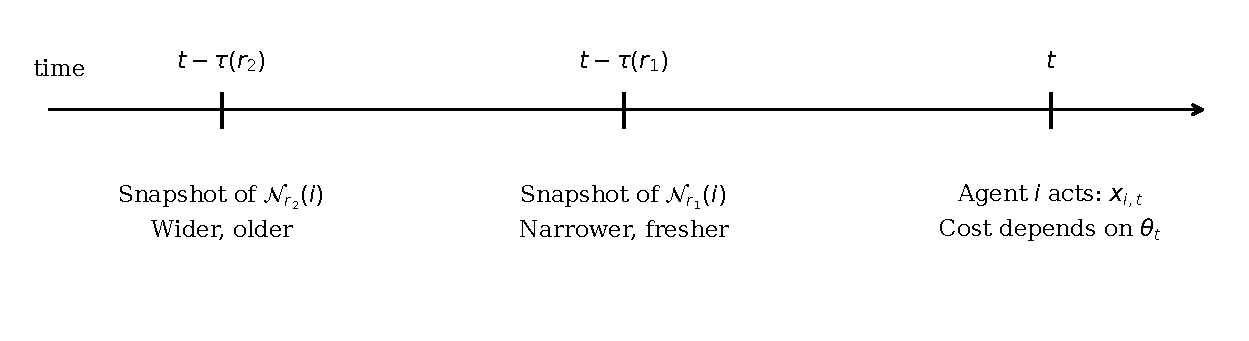
\includegraphics[width=\linewidth]{figures/snapshot_timing.pdf}
\caption{A radius-$r$ synchronized snapshot is taken at time $t-\tau(r)$ and
used for the decision at time $t$. For $r_2>r_1$ with $\tau(r_2)>\tau(r_1)$,
the wider snapshot is older. Cost is evaluated against the current state $\theta_t$.}
\label{fig:snapshot-timing}
\end{figure}
\begin{table}[htbp]
\centering\small
\setlength{\tabcolsep}{3pt}
\caption{Assumptions used in the derivations. All rows use square-integrable
targets and a deterministic positive-definite quadratic cost; normalized shares
require $R_\infty>0$. Entries describe the sufficient assumptions used by the
proofs, including their stated non-Gaussian extensions. ``Fixed epoch'' means
stationarity is unnecessary for that result.}
\label{tab:result-assumptions}
\begin{tabular}{@{}>{\raggedright\arraybackslash}p{.23\linewidth}>{\raggedright\arraybackslash}p{.12\linewidth}>{\raggedright\arraybackslash}p{.13\linewidth}>{\centering\arraybackslash}p{.095\linewidth}>{\centering\arraybackslash}p{.085\linewidth}>{\raggedright\arraybackslash}p{.275\linewidth}@{}}
\toprule
Result & Stationarity & Common-rate innovation & Affine target & Gaussian & Other \\
\midrule
Lemma~\ref{lem:radner_projection}; observation~\eqref{eq:general_crossover}
 & Fixed epoch & No & No & No & Admissible linear policy space \\
Lemma~\ref{lem:innovation_split}; Theorems~\ref{thm:OU_stale_regret}--\ref{thm:local_global_crossover}
 & Time & Yes & Yes & No & Scalar decay; finite-delay crossover as stated \\
Proposition~\ref{prop:aggregate_local}
 & Fixed epoch & No & Yes & No & Independent, mean-zero, equal-variance states \\
Threshold~\eqref{eq:aggregate_rho_star}
 & Time & Yes & Yes & No & Aggregate model plus temporal law \\
Theorem~\ref{thm:spatiotemporal_composition}
 & Time & Yes & Yes & No & Synchronized snapshots \\
Proposition~\ref{thm:marginal_balance}
 & Time & Yes & Yes & No & Differentiable $\tau,\eta_S$; $\eta_S<1$ \\
Lemma~\ref{prop:canonical_eta_S}
 & Space & No & Yes & Yes & $Q=qI$; exponential spatial covariance and kernel \\
Theorem~\ref{thm:canonical_optimal_radius}
 & Space/time & Yes & Yes & Yes & Canonical model and linear delay \\
\bottomrule
\end{tabular}
\end{table}

\subsection{Two Benchmark Architectures}
\label{subsec:two_architectures}

At decision time $t$, the \emph{fresh-local} architecture is
\begin{equation}
    \mathcal{A}_{\mathrm{loc}}
    =
    \left(
        \mathcal{G}^{\mathrm{loc}}_{1,t},
        \ldots,
        \mathcal{G}^{\mathrm{loc}}_{n,t}
    \right),
    \qquad
    \mathcal{G}^{\mathrm{loc}}_{i,t}
    =
    \sigma\!\left(
        \theta_{i,t}
    \right).
    \label{eq:sec3_local_arch}
\end{equation}
Its regret is
\begin{equation}
    R_{\mathrm{loc}}
    \triangleq
    R(\mathcal{A}_{\mathrm{loc}}).
    \label{eq:Rloc}
\end{equation}
Because this information is current, $R_{\mathrm{loc}}$ does not depend on
the global information delay $\tau$. Its magnitude instead reflects how much
of the full-information decision can be inferred from local information alone.

The \emph{stale-global} architecture at delay $\tau$ is
\begin{equation}
    \mathcal{A}_{\mathrm{glob}}(\tau)
    =
    \left(
        \mathcal{G}^{\tau}_t,\ldots,\mathcal{G}^{\tau}_t
    \right),
    \qquad
    \mathcal{G}^{\tau}_t
    \triangleq
    \sigma\!\left(
        \theta_{t-\tau}
    \right).
    \label{eq:sec3_global_arch}
\end{equation}
All agents therefore share the same complete but delayed snapshot of the
environment. We denote its regret by
\begin{equation}
    R_{\mathrm{glob}}(\tau)
    \triangleq
    R(\mathcal{A}_{\mathrm{glob}}(\tau)).
    \label{eq:Rglob}
\end{equation}

On a finite connected graph of diameter $D$, these are the $r=0$ and
$r=D$ members of the synchronized-snapshot family in
Section~\ref{sec:spatiotemporal_predictability}, with delays zero and
$\tau$, respectively.

For reference, define also the \emph{open-loop} architecture, whose decision is
the best constant, state-independent action. Its optimal action is
$\mathbb{E}[x_t^\star]$, and its regret is
\begin{equation}
    R_\infty
    \triangleq
    \frac{1}{2}
        \left\|
            x_t^\star-\mathbb{E}[x_t^\star]
        \right\|_Q^2.
    \label{eq:Rinf_general}
\end{equation}

The term \emph{open-loop} is borrowed from control, where it describes a controller that does not use measurements. Here it simply means a decision that ignores the state. The best such decision is the mean $\mathbb E[x^\star_t]$. For any constant $c$, the cross term vanishes because $x^\star_t-\mathbb E x^\star_t$ has mean zero and $Q$ is deterministic, so

\[
\|x^\star_t-c\|_Q^2=\|x^\star_t-\mathbb E x^\star_t\|_Q^2+(\mathbb E x^\star_t-c)^\top Q(\mathbb E x^\star_t-c).
\]

The second term is nonnegative and vanishes only at $c=\mathbb E x^\star_t$.

Throughout the normalized comparisons below we assume $R_\infty>0$, excluding the trivial case in
which the clairvoyant decision is deterministic.

Under $\mathcal A_{\rm glob}(\tau)$ every agent has the \emph{same} information $\sigma(\theta_{t-\tau})$. When information is common, the team problem collapses to a single-decision-maker problem (see Corollary~\ref{cor:conditional_normal_equations} and Appendix~\ref{app:toolkit-2}). The optimal joint policy is then the ordinary conditional expectation $\mathbb E[x^\star_t\mid\theta_{t-\tau}]$, even when $Q$ has off-diagonal blocks. Stale-global regret is therefore one-half the minimum $Q$-weighted mean-square error of predicting the \emph{current} full-information decision from the \emph{old} snapshot:

\[
2R_{\rm glob}(\tau)=\min_{g:\,g(\theta_{t-\tau})\in L^2}\ \big\|x^\star_t-g(\theta_{t-\tau})\big\|_Q^2 .
\]

Define the two loss shares as regret ratios:
\begin{equation}
    \eta_T(\tau)\triangleq\frac{R_{\mathrm{glob}}(\tau)}{R_\infty},
    \qquad 0\le\eta_T(\tau)\le1,
    \label{eq:temporal_unpredictability}
\end{equation}
and
\begin{equation}
    \eta_S(0)\triangleq\frac{R_{\mathrm{loc}}}{R_\infty},
    \qquad 0\le\eta_S(0)\le1.
    \label{eq:eta_S_local}
\end{equation}

Both shares lie in $[0,1]$. They are nonnegative because regret is nonnegative. They are at most one because constant actions are admissible under \emph{every} architecture: each agent can ignore its information and play its component of $\mathbb E[x^\star_t]$. So no architecture can do worse than open loop, and $R(\mathcal A)\le R_\infty$. We abbreviate $\eta_0\triangleq\eta_S(0)$. The argument "$0$" anticipates Section~\ref{sec:spatiotemporal_predictability}, where $\eta_S(r)$ is defined for every radius $r$ and radius zero is the fresh-local architecture.

The quantity $\eta_S(0)$ measures what is lost by restricting information
spatially, while $\eta_T(\tau)$ measures what is lost by allowing global
information to age. The captured local share is $1-\eta_S(0)$.
At zero delay, $\eta_T(0)=0$ because the complete current state determines
$x_t^\star$. The old snapshot becomes uninformative for this decision if $\mathbb E[x^\star_t\mid\theta_{t-\tau}]\to\mathbb E[x^\star_t]$ in mean square; in that case $\eta_T(\tau)\to1$. Strong mixing conditions (Appendix~\ref{app:glossary}) guarantee this.

One might expect $\eta_T$ to increase with $\tau$ automatically, but information monotonicity \eqref{eq:architecture_monotonicity} does not apply. For $0\le\tau_1<\tau_2$, the older snapshot $\theta_{t-\tau_2}$ is generally not a function of the newer one $\theta_{t-\tau_1}$, so the $\sigma$-algebras are not nested. For a \emph{Markov} environment, monotonicity does hold. Given $\theta_{t-\tau_1}$, the older value $\theta_{t-\tau_2}$ adds nothing about $\theta_t$. Predicting from $\theta_{t-\tau_2}$ alone is therefore no better than predicting from the pair $(\theta_{t-\tau_1},\theta_{t-\tau_2})$, which is exactly as good as predicting from $\theta_{t-\tau_1}$ alone. This is the \emph{data-processing inequality} for prediction error; the OU formula \eqref{eq:OU_etaT} below exhibits the monotonicity explicitly.

Dividing by $R_\infty>0$ gives the crossover observation
\begin{equation}
    R_{\mathrm{loc}}<R_{\mathrm{glob}}(\tau)
    \quad\Longleftrightarrow\quad
    \eta_T(\tau)>\eta_S(0).
    \label{eq:general_crossover}
\end{equation}
Fresh-local information is preferable precisely when the temporal information
lost by waiting for a global view exceeds the decision-relevant information
unavailable locally.

\subsection{Gauss--Markov Temporal Model}
\label{subsec:OU_model}

We now specialize the temporal unpredictability function to obtain a closed
form. Suppose the environment follows the stationary multivariate
Ornstein--Uhlenbeck process
\begin{equation}
    d\theta_t
    =
    -\frac{1}{T}
    \left(
        \theta_t-\bar{\theta}
    \right)dt
    +
    \sqrt{\frac{2}{T}}\,
    \Sigma_\infty^{1/2}dW_t,
    \label{eq:OU_process}
\end{equation}
where $T>0$ is the temporal coherence time,
$\bar{\theta}$ is the stationary mean, and $\Sigma_\infty$ is the stationary
covariance matrix. The process may exhibit arbitrary instantaneous
cross-correlation among agents through $\Sigma_\infty$; the simplifying
assumption is that all temporal modes share the same decay time $T$.

Readers unfamiliar with stochastic differential equations can read \eqref{eq:OU_process} as shorthand for three facts (derived in Appendix~\ref{app:toolkit-4}), which are all the paper uses:
\begin{enumerate}
\item $\theta_t$ is a stationary Gaussian process with mean $\bar\theta$ and covariance $\Sigma_\infty$.
\item $\operatorname{Cov}(\theta_t,\theta_s)=e^{-|t-s|/T}\Sigma_\infty$.
\item For every $\tau>0$ the decomposition \eqref{eq:state_innovation_decomposition} below holds, with an explicitly known innovation covariance.
\end{enumerate}

The drift $-(\theta_t-\bar\theta)/T$ pulls the state back toward its mean at rate $1/T$. The noise scale $\sqrt{2/T}$ is chosen exactly so that the stationary covariance equals $\Sigma_\infty$. The key simplification is that the drift is the \emph{scalar} $-1/T$ times the identity. Every component of $\theta$, and every linear combination of components (every "mode"), forgets its past at the same rate $1/T$. A general matrix drift would give different modes different coherence times; Section~\ref{sec:discussion_conclusions} discusses that case.

Assume further that
\begin{equation}
    b(\theta)=B\theta+b_0,
    \label{eq:affine_b}
\end{equation}
so that the full-information decision is affine:
\begin{equation}
    x^\star(\theta)
    =
    Q^{-1}B\theta+Q^{-1}b_0.
    \label{eq:affine_xstar}
\end{equation}

Let
\begin{equation}
    \rho
    \triangleq
    \frac{\tau}{T}
    \label{eq:rho_definition}
\end{equation}
denote the dimensionless staleness ratio.

The OU transition law \cite[eqs.~(8)--(10), (14)]{ornee2021ou} gives the decomposition

\begin{equation}
\theta_t-\bar\theta=e^{-\rho}(\theta_{t-\tau}-\bar\theta)+\varepsilon_{t,\tau},\qquad \mathbb E[\varepsilon_{t,\tau}\mid\theta_{t-\tau}]=0,\qquad \operatorname{Cov}(\varepsilon_{t,\tau})=(1-e^{-2\rho})\Sigma_\infty.
\label{eq:state_innovation_decomposition}
\end{equation}

We call $\varepsilon_{t,\tau}$ the \emph{innovation}: the part of the current state that cannot be predicted from the state $\tau$ time units earlier. For the OU process it is Gaussian and independent of $\{\theta_s:s\le t-\tau\}$. Its covariance follows from stationarity. The two terms in \eqref{eq:state_innovation_decomposition} are uncorrelated, so $\Sigma_\infty=\operatorname{Cov}(\theta_t)=e^{-2\rho}\Sigma_\infty+\operatorname{Cov}(\varepsilon_{t,\tau})$.

Define the centered full-information decision by
\begin{equation}
    \bar x^\star\triangleq\mathbb E[x_t^\star],
    \qquad X_t\triangleq x_t^\star-\bar x^\star.
    \label{eq:centered_clairvoyant_action}
\end{equation}
Because $x^\star(\theta)=K\theta+Q^{-1}b_0$ is affine, $\bar x^\star=K\bar\theta+Q^{-1}b_0$ and $X_t=K(\theta_t-\bar\theta)$. Applying $K$ to \eqref{eq:state_innovation_decomposition} gives

\begin{equation}
X_t=e^{-\rho}X_{t-\tau}+K\varepsilon_{t,\tau},\qquad K=Q^{-1}B.
\label{eq:xstar_innovation_decomposition}
\end{equation}

We may work with the centered target $X_t$ without loss of generality. If $u$ is admissible, so is $u-\bar x^\star$, since each agent can subtract a known constant. Moreover $(x^\star_t-\bar x^\star)-(u-\bar x^\star)=x^\star_t-u$. The shift $u\mapsto u-\bar x^\star$ is therefore a one-to-one map of the admissible set onto itself that leaves every error unchanged. Note also that $\|X_t\|_Q^2=2R_\infty$ by \eqref{eq:Rinf_general}.

We use the $L^2$ norm $\|Y\|_Q^2=\mathbb E[Y^\top QY]$ defined in
\eqref{eq:q_inner_product}.

\begin{lemma}[Innovation split]
\label{lem:innovation_split}
Under \eqref{eq:OU_process}--\eqref{eq:affine_b}, every square-integrable
$\mathbb R^d$-valued function $u$ of $\theta_{t-\tau}$ satisfies
\begin{equation}
    \|X_t-u\|_Q^2
    =\|e^{-\rho}X_{t-\tau}-u\|_Q^2
      +(1-e^{-2\rho})\,2R_\infty.
    \label{eq:innovation_split}
\end{equation}
\end{lemma}
\begin{proof}
Split the error into an "old" part and a "new" part:

\[
X_t-u=\underbrace{\big(e^{-\rho}X_{t-\tau}-u\big)}_{\triangleq\,A,\ \text{a function of }\theta_{t-\tau}}+\ K\varepsilon_{t,\tau}.
\]

\emph{Orthogonality.} Because $A$ is a function of $\theta_{t-\tau}$, the tower property (Appendix~\ref{app:toolkit-2}) gives

\[
\mathbb E\big[A^\top QK\varepsilon_{t,\tau}\big]=\mathbb E\big[A^\top QK\,\mathbb E[\varepsilon_{t,\tau}\mid\theta_{t-\tau}]\big]=0 .
\]

By Pythagoras, $\|X_t-u\|_Q^2=\|A\|_Q^2+\|K\varepsilon_{t,\tau}\|_Q^2$.

\emph{Size of the new part.} Setting $u=0$ in this identity gives $\|X_t\|_Q^2=e^{-2\rho}\|X_{t-\tau}\|_Q^2+\|K\varepsilon_{t,\tau}\|_Q^2$. Stationarity gives $\|X_{t-\tau}\|_Q^2=\|X_t\|_Q^2=2R_\infty$. Hence $\|K\varepsilon_{t,\tau}\|_Q^2=(1-e^{-2\rho})\,2R_\infty$.

Equivalently, using \eqref{eq:state_innovation_decomposition} directly: $\|K\varepsilon\|_Q^2=\operatorname{tr}\!\big(K^\top QK\operatorname{Cov}\varepsilon\big)=(1-e^{-2\rho})\operatorname{tr}(K^\top QK\Sigma_\infty)=(1-e^{-2\rho})\,2R_\infty$.
\end{proof}

The first term is the error in reproducing the predictable old decision;
the second is the fresh innovation that the old snapshot cannot predict.
For global information, the first error can be eliminated entirely.

\begin{theorem}[Exact stale-global regret]
\label{thm:OU_stale_regret}
Under \eqref{eq:OU_process}--\eqref{eq:affine_b},
\begin{equation}
    \boxed{
    R_{\mathrm{glob}}(\tau)
    =
    \left(
        1-e^{-2\tau/T}
    \right)R_\infty,
    }
    \label{eq:OU_exact_regret}
\end{equation}
where
\begin{equation}
    R_\infty
    =
    \frac{1}{2}
    \operatorname{tr}
    \left(
        B^\top Q^{-1}B\,
        \Sigma_\infty
    \right).
    \label{eq:OU_Rinf}
\end{equation}
Equivalently,
\begin{equation}
    \boxed{
    \eta_T(\tau)
    =
    1-e^{-2\tau/T}.
    }
    \label{eq:OU_etaT}
\end{equation}
\end{theorem}

\begin{proof}
The global snapshot allows any function of $\theta_{t-\tau}$. In particular it allows $u=e^{-\rho}X_{t-\tau}$, which makes the first term in \eqref{eq:innovation_split} zero. Since that term is nonnegative, this choice is optimal. In uncentered form, the optimal stale-global action is

\[
u^\star_{\rm glob}=\bar x^\star+e^{-\tau/T}\big(x^\star_{t-\tau}-\bar x^\star\big):
\]

the old full-information decision, shrunk toward its mean. Only the innovation term remains, so $2R_{\rm glob}(\tau)=(1-e^{-2\rho})\,2R_\infty$, which is \eqref{eq:OU_exact_regret}.

For \eqref{eq:OU_Rinf}, use the identity $\mathbb E[Y^\top AY]=\operatorname{tr}(A\operatorname{Cov}Y)$ for mean-zero $Y$ and the cyclic property of the trace (Appendix~\ref{app:toolkit-6}):

\[
\begin{aligned}
2R_\infty&=\mathbb E[X_t^\top QX_t]
=\operatorname{tr}\!\big(QK\Sigma_\infty K^\top\big)
=\operatorname{tr}\!\big(K^\top QK\,\Sigma_\infty\big),\\
K^\top QK&=B^\top Q^{-1}QQ^{-1}B=B^\top Q^{-1}B.
\end{aligned}
\]
\end{proof}

\textbf{Generality of the innovation argument.} The proof uses only three ingredients: stationarity, an affine decision, and a decomposition $\theta_t-\bar\theta=a(\theta_{t-\tau}-\bar\theta)+\varepsilon$ with a \emph{scalar} $a$ and $\mathbb E[\varepsilon\mid\theta_{t-\tau}]=0$. Neither Gaussianity nor full independence of $\varepsilon$ from the past is needed. For example, consider the discrete-time AR(1) process $\theta_k-\bar\theta=a(\theta_{k-1}-\bar\theta)+\varepsilon_k$ with $0<a<1$ and i.i.d. square-integrable mean-zero innovations independent of the past. It satisfies the decomposition at lag $k$ with $a^k$ in place of $e^{-\rho}$. Writing $a=e^{-1/T}$, with $T$ measured in time steps, gives $\eta_T(k)=1-a^{2k}=1-e^{-2k/T}$.

The result has a simple interpretation. When $\tau\ll T$, the environment
changes little over the information delay and
\begin{equation}
    R_{\mathrm{glob}}(\tau)
    =
    2\frac{\tau}{T}R_\infty
    +
    o\!\left(\frac{\tau}{T}\right).
    \label{eq:small_rho}
\end{equation}

Here we used $1-e^{-x}=x+O(x^2)$ with $x=2\tau/T$. The notation $o(\tau/T)$ denotes a term that becomes negligible relative to $\tau/T$ as $\tau/T\to0$ (Appendix~\ref{app:toolkit-7}).

When $\tau\gg T$, the delayed global snapshot becomes essentially uninformative about
the current decision and
\[
    R_{\mathrm{glob}}(\tau)
    \rightarrow
    R_\infty.
\]
Staleness therefore matters relative to the timescale on which
decision-relevant state changes.
For any fixed $\tau>0$, the same identity gives
$R_{\mathrm{glob}}(\tau)\to R_\infty$ as $T\downarrow0$ and
$R_{\mathrm{glob}}(\tau)\to0$ as $T\to\infty$.

\subsection{Fresh-Local versus Stale-Global Crossover}
\label{subsec:OU_crossover}

Combining the observation \eqref{eq:general_crossover} with
\eqref{eq:OU_etaT} yields the first main architectural result.

\begin{theorem}[Fresh-local versus stale-global crossover]
\label{thm:local_global_crossover}
Under the Gauss--Markov and affine-decision assumptions of
Theorem~\ref{thm:OU_stale_regret}, suppose
$0\le\eta_S(0)<1$. Fresh-local information strictly
outperforms stale-global information if and only if
\begin{equation}
    \boxed{
    \frac{\tau}{T}
    >
    \frac{1}{2}
    \log
    \frac{1}{1-\eta_S(0)}.
    }
    \label{eq:OU_crossover}
\end{equation}
Equivalently, defining
\begin{equation}
    \rho^\star
    \triangleq
    \frac{1}{2}
    \log
    \frac{1}{1-\eta_S(0)},
    \label{eq:rho_star_general}
\end{equation}
we have
\begin{equation}
    R_{\mathrm{loc}}
    <
    R_{\mathrm{glob}}(\tau)
    \quad\Longleftrightarrow\quad
    \rho>\rho^\star.
    \label{eq:rho_crossover}
\end{equation}
\emph{If $\eta_S(0)=1$, we set $\rho^\star=+\infty$: no finite delay makes fresh-local information strictly better.}

\end{theorem}

\begin{proof}
By \eqref{eq:general_crossover}, fresh-local wins exactly when
\[
    1-e^{-2\rho}
    >
    \eta_S(0).
\]
Equivalently,
\[
    e^{-2\rho}
    <
    1-\eta_S(0),
\]
which gives \eqref{eq:OU_crossover}.
\end{proof}

\emph{Why a single threshold?} $R_{\rm loc}$ depends only on the distribution of the state at a single time. With the one-time state distribution held fixed, it involves neither the delay $\tau$ nor the coherence time $T$, because local information is current. All dependence on staleness is in $R_{\rm glob}(\tau)$, which increases in $\tau$. For $0<\eta_S(0)<1$, the comparison is a flat line crossed once by an increasing curve. When $\eta_S(0)=0$, equality occurs at zero delay; when $\eta_S(0)=1$, there is no finite crossing.


The limiting cases are informative. If
\[
    \eta_S(0)=0,
\]
fresh-local information is sufficient to reproduce the full-information
decision, and the fresh-local architecture dominates for every $\tau>0$. If
\[
    \eta_S(0)=1,
\]
local information provides no improvement over open loop, and stale-global
information is never strictly worse at any finite delay.

More generally, Theorem~\ref{thm:local_global_crossover} identifies two
dimensionless determinants of the architecture choice. The staleness ratio
$\tau/T$ measures the loss of temporal relevance incurred by global
information, while $\eta_S(0)$ measures the share of decision-relevant
variation omitted locally. Within the comparison of the two
pure benchmarks, fresh-local has lower regret precisely when the two loss
fractions cross.

\subsection{Role of Decision Coupling}
\label{subsec:coupling_example}

The fresh-local omission share $\eta_S(0)$ depends jointly on the
spatial statistics of the environment and on the coupling structure of the
decision problem. To isolate the role of decision coupling, consider a
symmetric shared-resource model with $n\ge2$ scalar actions,
\begin{equation}
    f(x,\theta)
    =
    \sum_{i=1}^{n}
    \left(
        \frac{q}{2}x_i^2-\theta_i x_i
    \right)
    +
    \frac{\gamma}{2}
    \left(
        \sum_{i=1}^{n}x_i
    \right)^2,
    \qquad
    q>0,\;\gamma\ge0.
    \label{eq:shared_resource_cost}
\end{equation}
Here $q$ determines the local curvature or stiffness of each decision, while
$\gamma$ determines the strength of the shared coordination penalty. In the
notation of Section~\ref{sec:model},
\begin{equation}
    Q
    =
    qI+\gamma\mathbf{1}\mathbf{1}^\top,
    \qquad
    b(\theta)=\theta.
    \label{eq:shared_resource_Q}
\end{equation}

Here $\mathbf 1\in\mathbb R^n$ is the all-ones vector, so $\mathbf 1\mathbf 1^\top$ is the $n\times n$ all-ones matrix and $\mathbf 1^\top x=\sum_i x_i$. Expanding confirms that \eqref{eq:shared_resource_Q} matches \eqref{eq:shared_resource_cost}:

\[
\tfrac12x^\top(qI+\gamma\mathbf 1\mathbf 1^\top)x=\tfrac q2\sum_i x_i^2+\tfrac\gamma2\Big(\sum_i x_i\Big)^2 .
\]


Assume that the state components $\theta_i$ are independent, mean-zero
stationary OU processes with common variance $\sigma^2$ and common coherence
time $T$.

The full-information action is $x^\star=Q^{-1}\theta$. The inverse of an "identity plus rank-one" matrix has a closed form (Sherman--Morrison, Appendix~\ref{app:toolkit-6}):

\[
\big(qI+\gamma\mathbf 1\mathbf 1^\top\big)^{-1}=\frac1q\Big(I-\frac{\gamma}{q+\gamma n}\mathbf 1\mathbf 1^\top\Big),
\]

which can be checked by multiplying out. Applying it to $\theta$ gives

\begin{equation}
    x_i^\star
    =
    \frac{\theta_i}{q}
    -
    \frac{\gamma}
    {q(q+\gamma n)}
    \sum_{j=1}^{n}\theta_j.
    \label{eq:shared_resource_xstar}
\end{equation}
Thus, even though the linear reward $\theta_i x_i$ is local, coupling through
the common resource makes agent $i$'s optimal action depend on the states of
all other agents.

\begin{proposition}[Local explainability under aggregate coupling]
\label{prop:aggregate_local}
For the model \eqref{eq:shared_resource_cost}, the optimal fresh-local policy
is
\begin{equation}
    u_i^{\mathrm{loc}}
    =
    \frac{\theta_i}{q+\gamma},
    \label{eq:optimal_local_shared}
\end{equation}
and
\begin{align}
    R_\infty
    &=
    \frac{
        n\sigma^2
        \left(
            q+\gamma(n-1)
        \right)
    }{
        2q(q+\gamma n)
    },
    \label{eq:aggregate_Rinf}
    \\
    R_{\mathrm{loc}}
    &=
    \frac{
        n\sigma^2\gamma^2(n-1)
    }{
        2q(q+\gamma)(q+\gamma n)
    }.
    \label{eq:aggregate_Rloc}
\end{align}
Consequently, the fresh-local omission share is
\begin{equation}
    \boxed{
    \eta_S(0)
    =
    \frac{
        \gamma^2(n-1)
    }{
        (q+\gamma)
        \left(
            q+\gamma(n-1)
        \right)
    }.
    }
    \label{eq:aggregate_eta}
\end{equation}
\end{proposition}

\emph{Intuition for \eqref{eq:optimal_local_shared}.} Agent $i$ sees only $\theta_i$. Remote states are independent of $\theta_i$ and have mean zero, and the optimal rules below have zero means. Agent $i$ therefore expects each other optimal action to be zero on average. Its own action, however, enters the aggregate penalty $\tfrac\gamma2(\sum_j x_j)^2$ directly and adds $\gamma x_i$ to its marginal cost. Its effective stiffness is therefore $q+\gamma$ rather than $q$. The full-information action \eqref{eq:shared_resource_xstar} differs because it also reacts to the realized aggregate $\sum_j\theta_j$, which agent $i$ cannot see.


\begin{proof}
Recall the coupled normal equations \eqref{eq:block_conditional_normal_equations}:
\[
 Q_{ii}u_i+\sum_{j\ne i}Q_{ij}\mathbb E[u_j\mid\mathcal G_i]
 =\mathbb E[b_i(\theta_t)\mid\mathcal G_i].
\]
Here $Q_{ii}=q+\gamma$, $Q_{ij}=\gamma$ for $j\ne i$, and $b_i(\theta)=\theta_i$.
Let $\mu_j=\mathbb E[u_j]$. For $j\ne i$, the policy $u_j$ is a function of $\theta_{j,t}$,
which is independent of $\theta_{i,t}$, so
\[
\mathbb E[u_j\mid\mathcal G^{\mathrm{loc}}_{i,t}]
=\mathbb E[u_j]=\mu_j,
\]
while $\theta_{i,t}$ is
$\mathcal G^{\mathrm{loc}}_{i,t}$-measurable. The conditional normal equation
\eqref{eq:block_conditional_normal_equations} therefore gives
\[
(q+\gamma)u_i
+\gamma\sum_{j\ne i}\mu_j
-\theta_{i,t}=0.
\]
Taking expectations yields
\[
q\mu_i+\gamma\sum_j\mu_j=0.
\]
Summing over $i$ implies $\sum_j\mu_j=0$, hence every $\mu_i=0$ and
$u_i=\theta_{i,t}/(q+\gamma)$, which proves
\eqref{eq:optimal_local_shared}. This argument uses independence, zero means,
square integrability, and strict convexity; Gaussianity is not required for the
local-policy formula.

\emph{Open-loop regret.} Here $B=I$ and $\Sigma_\infty=\sigma^2I$, so by \eqref{eq:OU_Rinf}, $R_\infty=\tfrac{\sigma^2}2\operatorname{tr}(Q^{-1})$. From the Sherman--Morrison formula above,

\[
\operatorname{tr}(Q^{-1})=\frac1q\Big(n-\frac{\gamma n}{q+\gamma n}\Big)=\frac{n\,(q+\gamma(n-1))}{q\,(q+\gamma n)},
\]

which gives \eqref{eq:aggregate_Rinf}.

\emph{Local regret.} By the Pythagorean form of Lemma~\ref{lem:radner_projection} (the consequences following Lemma~\ref{lem:radner_projection}, with both $x^\star$ and $u^{\rm loc}$ mean zero), $2R_{\rm loc}=\|x^\star\|_Q^2-\|u^{\rm loc}\|_Q^2=2R_\infty-\|u^{\rm loc}\|_Q^2$. Since $u^{\rm loc}=\theta/(q+\gamma)$ and $\operatorname{tr}(Q)=n(q+\gamma)$,

\[
\|u^{\rm loc}\|_Q^2=\frac{\sigma^2\operatorname{tr}(Q)}{(q+\gamma)^2}=\frac{n\sigma^2}{q+\gamma}.
\]

Therefore

\[
R_{\rm loc}=\frac{n\sigma^2}{2}\left[\frac{q+\gamma(n-1)}{q(q+\gamma n)}-\frac{1}{q+\gamma}\right]=\frac{n\sigma^2}{2}\cdot\frac{(q+\gamma(n-1))(q+\gamma)-q(q+\gamma n)}{q(q+\gamma)(q+\gamma n)} .
\]

The numerator reduces to $\gamma^2(n-1)$, which gives \eqref{eq:aggregate_Rloc}.

\emph{Share.} Dividing \eqref{eq:aggregate_Rloc} by \eqref{eq:aggregate_Rinf}, the factors $n\sigma^2/2$ and $q(q+\gamma n)$ cancel, leaving \eqref{eq:aggregate_eta}.

\end{proof}

Combining Proposition~\ref{prop:aggregate_local} with
Theorem~\ref{thm:local_global_crossover} gives an explicit threshold.
From \eqref{eq:aggregate_eta},

\[
1-\eta_S(0)=\frac{(q+\gamma)(q+\gamma(n-1))-\gamma^2(n-1)}{(q+\gamma)(q+\gamma(n-1))}=\frac{q\,(q+\gamma n)}{(q+\gamma)(q+\gamma(n-1))},
\]

because the numerator expands to $q^2+q\gamma(n-1)+q\gamma=q(q+\gamma n)$. Substituting into \eqref{eq:rho_star_general} gives

\begin{equation}
    \boxed{
    \rho^\star(\gamma,n)
    =
    \frac{1}{2}
    \log
    \left[
        \frac{
            (q+\gamma)
            \left(
                q+\gamma(n-1)
            \right)
        }{
            q(q+\gamma n)
        }
    \right].
    }
    \label{eq:aggregate_rho_star}
\end{equation}
Therefore
\begin{equation}
    R_{\mathrm{loc}}
    <
    R_{\mathrm{glob}}(\tau)
    \quad\Longleftrightarrow\quad
    \frac{\tau}{T}
    >
    \rho^\star(\gamma,n).
    \label{eq:aggregate_crossover}
\end{equation}

As $n\rightarrow\infty$,
\begin{equation}
    \boxed{
    \rho^\star(\gamma,n)
    \longrightarrow
    \frac{1}{2}
    \log
    \left(
        1+\frac{\gamma}{q}
    \right).
    }
    \label{eq:large_n_threshold}
\end{equation}

To see the limit, write the ratio in \eqref{eq:aggregate_rho_star} as $\frac{q+\gamma}{q}\cdot\frac{q+\gamma(n-1)}{q+\gamma n}$; the second factor tends to one. Equivalently, \eqref{eq:aggregate_eta} gives $\eta_S(0)\to\gamma/(q+\gamma)$. In a large system, local information explains the share $q/(q+\gamma)$ of decision variance. It misses the share $\gamma/(q+\gamma)$ driven by the aggregate, which requires nonlocal information to capture fully.

The local--global architecture choice therefore collapses, in the
large-system limit, to a comparison between two dimensionless quantities:
\begin{equation}
    \boxed{
    \underbrace{\frac{\tau}{T}}_{\text{information staleness}}
    \qquad\text{and}\qquad
    \underbrace{
        \frac{1}{2}
        \log
        \left(
            1+\frac{\gamma}{q}
        \right)
    }_{\text{value of coordination}}.
    }
    \label{eq:two_dimensionless_quantities}
\end{equation}

The label "value of coordination" is interpretive, not a separate result. $\tfrac12\log(1+\gamma/q)$ is the staleness at which a global snapshot's temporal loss equals $\gamma/(q+\gamma)$, the large-$n$ share of decision variance unavailable to the fresh-local architecture.


When $\gamma=0$, the decisions decouple and
$\eta_S(0)=0$: current local information is sufficient, so any
positive global delay makes the fresh-local architecture preferable. As $\gamma$
increases, each agent's optimal action depends more strongly on remote states,
$\eta_S(0)$ increases, and the crossover moves to larger
$\tau/T$. Thus stronger coordination coupling makes the system willing to
tolerate increasingly stale-global information before abandoning global
coordination in favor of fresh-local decisions.

The result provides the first endpoint characterization of the broader
freshness--scope problem. The next sections move beyond the binary
local--global comparison by allowing the information radius itself to vary,
and ask how spatial predictability and temporal staleness jointly determine
the optimal coordination scale.



\section{Spatial and Temporal Predictability}
\label{sec:spatiotemporal_predictability}

We now introduce intermediate architectures in which each agent observes a
synchronized snapshot within radius $r$. Temporal predictability determines
the freshness loss, while decision-relevant spatial predictability determines
the omission loss.

\subsection{Spatial Structure of the Environment}
\label{subsec:spatial_structure}

We first describe the spatial statistics that determine what nearby
observations reveal about remote state.

For simplicity of exposition, first suppose that each node has a scalar local
state, so that
\[
    \theta_t
    =
    (\theta_{1,t},\ldots,\theta_{n,t})^\top.
\]
The vector-valued case follows by replacing scalar covariances with block
covariances.

Let
\begin{equation}
    \bar{\theta}
    \triangleq
    \mathbb{E}[\theta_t],
    \qquad
    \Sigma_S
    \triangleq
    \operatorname{Cov}(\theta_t)
    \succeq 0
    \label{eq:spatial_covariance_general}
\end{equation}
denote the stationary mean and spatial covariance. The entry
$(\Sigma_S)_{ij}$ measures the instantaneous statistical dependence between
the states associated with nodes $i$ and $j$.

On a path, line, or Euclidean spatial domain, a canonical covariance model is
\begin{equation}
    \operatorname{Cov}
    \left(
        \theta_{i,t},
        \theta_{j,t}
    \right)
    =
    \sigma^2
    \exp
    \left(
        -\frac{d_G(i,j)}{\ell_s}
    \right),
    \label{eq:spatial_exponential_covariance}
\end{equation}
where $\ell_s>0$ is a spatial correlation length. Larger $\ell_s$ means that
states remain strongly correlated over greater network distance. In one
spatial dimension, \eqref{eq:spatial_exponential_covariance} is the
exponential, or Ornstein--Uhlenbeck, covariance model
\cite{williams2006gaussian}.

The kernel in \eqref{eq:spatial_exponential_covariance} is the same exponential that describes the OU process in time \eqref{eq:separable_space_time_covariance}, now applied in space. On a line this is more than an analogy. A Gaussian field with covariance $\sigma^2e^{-|z-z'|/\ell_s}$ \emph{is} a stationary OU process indexed by position $z$, and it therefore has the \textbf{spatial Markov property}: given the value at a point $z_0$, the field to the left of $z_0$ and the field to the right are independent. As a consequence, observing a segment tells you about the field outside it only through the segment's nearest endpoint. Lemma~\ref{prop:canonical_eta_S} relies on exactly this. On general graphs the analogous objects are Gaussian Markov random fields (Appendix~\ref{app:toolkit-5}).

\subsection{Temporal Structure}
\label{subsec:temporal_structure}

We use the common-rate model \eqref{eq:OU_process} with
$\Sigma_\infty=\Sigma_S$. Its stationary space-time covariance is
\begin{equation}
    \operatorname{Cov}(\theta_t,\theta_s)
    =e^{-|t-s|/T}\Sigma_S.
    \label{eq:separable_space_time_covariance}
\end{equation}

A space--time covariance is \emph{separable} if it factors as (a function of time lag) $\times$ (a spatial covariance), as in \eqref{eq:separable_space_time_covariance}. Here it means that every spatial covariance mode has the same normalized temporal correlation. Many physical fields are \emph{nonseparable}: for example, large-scale patterns may persist longer than small-scale ones \cite{gneiting2002nonseparable}. Section~\ref{sec:discussion_conclusions} discusses the consequences.

Thus $\Sigma_S$ specifies instantaneous spatial dependence and $T$ specifies
a common temporal coherence time; general nonseparable models need not have
this factorization \cite{gneiting2002nonseparable}.

\subsection{Snapshot Architectures}
\label{subsec:joint_spatiotemporal}

For radius $r$, define the zero-delay information available to agent $i$ at
time $t$ as
\begin{equation}
    \mathcal{I}_{i,t}^{(r)}
    \triangleq
    \sigma\!\left(
        \theta_{j,t}:j\in\mathcal{N}_r(i)
    \right).
    \label{eq:zero_delay_radius_information}
\end{equation}

$\mathcal I^{(r)}_{i,t}$ is the $\sigma$-algebra $\mathcal G^{(r)}_{i,t}$ of \eqref{eq:radius_arch} with the delay set to zero. We use a separate symbol because, in this section, the delay $\tau$ is a free parameter rather than the latency law $\tau(r)$. Section~\ref{sec:optimal_coordination_scale} reconnects them by setting $\tau=\tau(r)$.

The corresponding zero-delay radius-$r$ architecture is
\begin{equation}
    \mathcal{A}_{r,0}
    \triangleq
    \left(
        \mathcal{I}_{1,t}^{(r)},
        \ldots,
        \mathcal{I}_{n,t}^{(r)}
    \right).
    \label{eq:zero_delay_radius_architecture}
\end{equation}

A delayed synchronized-snapshot radius-$r$ architecture provides the same type
of information, shifted backward by $\tau$:
\begin{equation}
    \mathcal{A}_{r,\tau}
    \triangleq
    \left(
        \mathcal{I}_{1,t-\tau}^{(r)},
        \ldots,
        \mathcal{I}_{n,t-\tau}^{(r)}
    \right).
    \label{eq:delayed_radius_architecture}
\end{equation}
Such common-time snapshots arise, for example, when a coordinated optimizer
requires a temporally consistent system estimate at a common decision epoch, or
when asynchronous measurements cannot be combined without explicit time
alignment into a coherent state vector.
Define the normalized zero-delay spatial omission function
\begin{equation}
    \eta_S(r)
    \triangleq
    \frac{
        R(\mathcal{A}_{r,0})
    }{
        R_\infty
    }.
    \label{eq:eta_S_definition}
\end{equation}
The quantity $\eta_S(r)$ is the fraction of decision-relevant variation that
cannot be captured using current information within radius $r$.

Since zero-delay radius architectures are nested,
\begin{equation}
    r_2\ge r_1
    \quad\Longrightarrow\quad
    \mathcal{S}(\mathcal{A}_{r_1,0})
    \subseteq
    \mathcal{S}(\mathcal{A}_{r_2,0}),
    \label{eq:radius_architecture_nested}
\end{equation}

Nesting holds because $\mathcal N_{r_1}(i)\subseteq \mathcal N_{r_2}(i)$ whenever $r_1\le r_2$, and both snapshots carry the same time stamp. Information monotonicity \eqref{eq:architecture_monotonicity} therefore gives
\begin{equation}
    0
    \le
    \eta_S(r_2)
    \le
    \eta_S(r_1)
    \le
    1.
    \label{eq:eta_S_monotone}
\end{equation}
If radius zero observes precisely the local current component, then
\begin{equation}
    \eta_S(0)
    =
    \frac{R_{\mathrm{loc}}}{R_\infty}.
    \label{eq:eta_S_zero}
\end{equation}
On a finite connected graph with diameter $D$, complete current state is available at
$r=D$, so
\begin{equation}
    \eta_S(D)=0.
    \label{eq:eta_S_diameter}
\end{equation}

\subsection{Decision-Relevant Smoothness}
\label{subsec:decision_relevant_smoothness}

Suppose, as in \eqref{eq:affine_map_and_sensitivity}, that
\begin{equation}
    b(\theta)
    =
    B\theta+b_0.
    \label{eq:affine_b_spatial}
\end{equation}
Then
\begin{equation}
    x_t^\star
    =
    K\theta_t+k_0,
    \qquad
    K\triangleq Q^{-1}B,
    \qquad
    k_0\triangleq Q^{-1}b_0.
    \label{eq:decision_sensitivity_operator}
\end{equation}
The matrix $K$ is the decision-sensitivity operator: its block $K_{ij}$
describes how the state at node $j$ influences the full-information decision
at node $i$.

The covariance of the clairvoyant decision is
\begin{equation}
    \Sigma_x
    \triangleq
    \operatorname{Cov}(x_t^\star)
    =
    K\Sigma_S K^\top.
    \label{eq:decision_covariance}
\end{equation}
The function $\eta_S(r)$ therefore depends on four ingredients at once: (i) the state covariance $\Sigma_S$; (ii) the decision-sensitivity operator $K$; (iii) the cost metric $Q$; and (iv) the observation geometry $\{\mathcal N_r(i)\}$.

A spatial correlation length alone does not determine regret. By a \emph{mode} we mean a direction $\xi$ in state space, representing a spatial pattern of variation, such as an eigenvector of $\Sigma_S$. A pattern in the null space of $K$ ($K\xi=0$) changes the state without changing the desired decision, so residual uncertainty confined to that direction contributes no decision error. Conversely, a pattern with large $\sqrt{(K\xi)^\top Q(K\xi)}$ is amplified into the decision, so even small residual uncertainty about it can dominate regret. Experiment 5 illustrates this dependence with the covariance held fixed.

\begin{theorem}[Spatio-temporal predictability composition law]
\label{thm:spatiotemporal_composition}
Suppose the environment follows \eqref{eq:OU_process} with
$\Sigma_\infty=\Sigma_S$, and the full-information decision is affine
as in \eqref{eq:decision_sensitivity_operator}. For the snapshot family
\eqref{eq:delayed_radius_architecture}, every radius $r$ and finite delay
$\tau\ge0$ satisfy
\begin{equation}
    \boxed{
    R(\mathcal{A}_{r,\tau})
    =
    \left(
        1-e^{-2\tau/T}
    \right)R_\infty
    +
    e^{-2\tau/T}
    R(\mathcal{A}_{r,0}).
    }
    \label{eq:regret_composition_unnormalized}
\end{equation}
Equivalently,
\begin{equation}
    \boxed{
    \frac{
        R(\mathcal{A}_{r,\tau})
    }{
        R_\infty
    }
    =
    1
    -
    e^{-2\tau/T}
    \left(
        1-\eta_S(r)
    \right).
    }
    \label{eq:regret_composition_normalized}
\end{equation}
In terms of the temporal unpredictability
$\eta_T(\tau)=1-e^{-2\tau/T}$,
\begin{equation}
    \boxed{
    \eta_{ST}(r,\tau)
    =
    \eta_T(\tau)
    +
    \left(
        1-\eta_T(\tau)
    \right)
    \eta_S(r),
    }
    \label{eq:eta_ST_composition}
\end{equation}
where
\[
    \eta_{ST}(r,\tau)
    \triangleq
    \frac{
        R(\mathcal{A}_{r,\tau})
    }{
        R_\infty
    }.
\]
\end{theorem}

\textbf{Explained shares multiply.} Subtracting \eqref{eq:eta_ST_composition} from one gives the cleanest reading of the composition law:

\[
1-\eta_{ST}(r,\tau)=\big(1-\eta_T(\tau)\big)\big(1-\eta_S(r)\big)=e^{-2\tau/T}\big(1-\eta_S(r)\big).
\]

The share of the decision that a delayed snapshot explains is the share that survives the delay times the share its spatial scope captures. Temporal and spatial losses do not simply add; the retained shares multiply. Section~\ref{sec:optimal_coordination_scale} optimizes exactly this product.


\begin{proof}
\textbf{Step 1 (centering).} As in Section~\ref{subsec:OU_model}, subtract $\bar x^\star$ from the target and from each admissible policy. This preserves admissibility and leaves every error unchanged.

\textbf{Step 2 (reduce to Lemma~\ref{lem:innovation_split}).} Under $\mathcal A_{r,\tau}$, agent $i$'s policy is a function of $\{\theta_{j,t-\tau}:j\in \mathcal N_r(i)\}$, a subset of $\theta_{t-\tau}$. The joint policy $u$ is therefore a function of $\theta_{t-\tau}$, and Lemma~\ref{lem:innovation_split} applies:

\[
\|X_t-u\|_Q^2=\|e^{-\rho}X_{t-\tau}-u\|_Q^2+(1-e^{-2\rho})\,2R_\infty .
\]

The second term does not depend on $u$, so only the first term is minimized.

\textbf{Step 3 (rescale).} Write $u=e^{-\rho}\tilde u$. The admissible set is a linear subspace and $e^{-\rho}\neq0$. Hence $u$ is admissible exactly when $\tilde u$ is, and $\tilde u_i$ depends on the same variables as $u_i$. Then

\[
\|e^{-\rho}X_{t-\tau}-e^{-\rho}\tilde u\|_Q^2=e^{-2\rho}\,\|X_{t-\tau}-\tilde u\|_Q^2 .
\]


\textbf{Step 4 (stationarity).} Minimizing $\|X_{t-\tau}-\tilde u\|_Q^2$ over $\tilde u$ is precisely the zero-delay radius-$r$ problem posed at time $t-\tau$: predict the decision at $t-\tau$ from neighborhood data at $t-\tau$. By stationarity its minimum equals the same problem's minimum at time $t$, namely $2R(\mathcal A_{r,0})$.

\textbf{Step 5 (combine).} $2R(\mathcal A_{r,\tau})=e^{-2\rho}\,2R(\mathcal A_{r,0})+(1-e^{-2\rho})\,2R_\infty$. Dividing by two gives \eqref{eq:regret_composition_unnormalized}; dividing further by $R_\infty$ gives \eqref{eq:regret_composition_normalized}--\eqref{eq:eta_ST_composition}.
\end{proof}

Theorem~\ref{thm:OU_stale_regret} is the case $r=D$ on a finite connected
graph, where $\eta_S(D)=0$. The temporal term
$(1-e^{-2\tau/T})R_\infty$ is the innovation that the delayed snapshot
cannot predict. The remaining spatial omission is discounted by
$e^{-2\tau/T}$, so broader information helps only with the part of the
current decision that remains temporally predictable.

\textbf{Generality of the composition law.} The proof of \eqref{eq:regret_composition_unnormalized} uses only the conditionally mean-zero, common-rate innovation of Lemma~\ref{lem:innovation_split}; Gaussianity is not needed. In the calculations below, Gaussianity lets us compute spatial prediction errors from covariances. For jointly Gaussian variables, the conditional mean is affine (linear after centering) and the conditional covariance is a Schur complement (Appendix~\ref{app:toolkit-3}). In the canonical model and Experiments 5--6, the cost matrix is $Q=qI$ or $I$, so there is no action coupling and each agent's optimal policy is simply its own conditional mean $\mathbb E[x^\star_i\mid\mathcal G_i]$. When $Q$ has off-diagonal blocks, \eqref{eq:regret_composition_unnormalized} still holds, but $\eta_S(r)$ must be computed from the \emph{joint} team solution of the coupled normal equations \eqref{eq:block_conditional_normal_equations} rather than agent by agent.

\section{Optimal Coordination Scale}
\label{sec:optimal_coordination_scale}

We now make information radius an architectural design variable. For each
$r$, an agent may base its action on observations available within radius $r$,
but those observations arrive after latency $\tau(r)$. The objective is to
select the spatial scope that minimizes architecture regret.

On a graph, admissible radii are generally integers. We first analyze the
continuous relaxation $r\in[0,D]$, where $D$ is the maximum allowed
information radius. On a finite graph, the exact optimizer is obtained by
minimizing over the admissible integer radii. Rounding the continuous optimum
to a neighboring integer is justified only when the interpolated regret curve
is unimodal.

\emph{Unimodal} means that the curve decreases up to a single minimum and increases after it. In that case the best integer radius is one of the two integers bracketing the continuous optimum $r^\star$, so it suffices to compare $R(\lfloor r^\star\rfloor)$ and $R(\lceil r^\star\rceil)$. If the curve has several local minima, the best integer can lie in a different valley altogether.

\subsection{Radius Family and Marginal Balance}
\label{subsec:radius_dependent_architectures}

We now formalize the radius family and the latency law that couples scope to
age.

Let
\begin{equation}
    \tau:
    [0,D]
    \rightarrow
    [0,\infty)
    \label{eq:latency_function_domain}
\end{equation}

Where a delay is a free parameter we write $\tau$; where it is determined by radius we write $\tau(r)$.

be a nondecreasing information-propagation law satisfying
\begin{equation}
    \tau(0)=0.
    \label{eq:tau_zero}
\end{equation}
Architecture $\mathcal{A}_{r,\tau(r)}$ provides each agent with information
from a synchronized radius-$r$ snapshot delayed by $\tau(r)$.

Why is an interior optimum possible at all? If the radius family were \emph{nested}, meaning that a larger radius always provided everything a smaller one did at the same age, then by \eqref{eq:architecture_monotonicity} regret could only decrease with radius, and the largest radius would always be an optimum. A strict interior optimum would then require charging explicitly for information. The synchronized-snapshot family avoids this because it is generally non-nested. At radius $r_2>r_1$, agent $i$ gives up the fresher values $\theta_{j,t-\tau(r_1)}$, $j\in \mathcal N_{r_1}(i)$, in exchange for older values over a wider neighborhood.

Define
\begin{equation}
    R(r)
    \triangleq
    R
    \left(
        \mathcal{A}_{r,\tau(r)}
    \right).
    \label{eq:R_of_r}
\end{equation}

We write $R(r)$ as shorthand for $R(\mathcal A_{r,\tau(r)})$ when the latency law is fixed.

By Theorem~\ref{thm:spatiotemporal_composition},
\begin{equation}
    \boxed{
    R(r)
    =
    R_\infty
    \left[
        1
        -
        e^{-2\tau(r)/T}
        \left(
            1-\eta_S(r)
        \right)
    \right].
    }
    \label{eq:radius_regret_master}
\end{equation}

On a finite graph, moving from radius $r$ to $r+1$ strictly improves
performance exactly when
\begin{equation}
e^{-2\tau(r+1)/T}\bigl(1-\eta_S(r+1)\bigr)
>
e^{-2\tau(r)/T}\bigl(1-\eta_S(r)\bigr),
\label{eq:discrete_radius_improvement}
\end{equation}
or, provided $1-\eta_S(r)>0$, equivalently
\begin{equation}
\log\!\left(
\frac{1-\eta_S(r+1)}{1-\eta_S(r)}
\right)
>
\frac{2\bigl(\tau(r+1)-\tau(r)\bigr)}{T}.
\label{eq:discrete_radius_log_improvement}
\end{equation}

Inequality \eqref{eq:discrete_radius_log_improvement} is \eqref{eq:discrete_radius_improvement} with logarithms taken of both sides and the terms rearranged. If $1-\eta_S(r)=0$ (radius $r$ explains nothing), the logarithm is undefined. Condition \eqref{eq:discrete_radius_improvement} then simply says that moving to $r+1$ helps if and only if $1-\eta_S(r+1)>0$.

The multiplicative comparison \eqref{eq:discrete_radius_improvement} remains
the primary statement when $1-\eta_S(r)=0$. Increasing the radius by one hop is
beneficial precisely when the discrete
proportional gain in decision-relevant spatial information exceeds the
freshness loss incurred over that hop.

At radius zero,
\begin{equation}
    R(0)
    =
    R_\infty\eta_S(0)
    =
    R_{\mathrm{loc}}.
    \label{eq:radius_zero_local}
\end{equation}
On a finite graph, if $D=\operatorname{diam}(G)$ and radius $D$ provides the
entire state, then
\begin{equation}
    R(D)
    =
    R_\infty
    \left(
        1-e^{-2\tau(D)/T}
    \right)
    =
    R_{\mathrm{glob}}(\tau(D)).
    \label{eq:radius_D_global}
\end{equation}
Equation~\eqref{eq:radius_regret_master} can be written as
\begin{equation}
    R(r)
    =
    R_T(r)+R_S(r),
    \label{eq:R_decomposition}
\end{equation}
where
\begin{align}
    R_T(r)
    &\triangleq
    \left(
        1-e^{-2\tau(r)/T}
    \right)R_\infty,
    \label{eq:temporal_component}
    \\
    R_S(r)
    &\triangleq
    e^{-2\tau(r)/T}
    \eta_S(r)R_\infty.
    \label{eq:spatial_component}
\end{align}
The temporal term increases with information radius whenever $\tau(r)$ does.
The zero-delay spatial omission fraction $\eta_S(r)$ decreases with radius,
although its contribution is discounted by the temporal relevance factor
$e^{-2\tau(r)/T}$.

The marginal rates below come from the multiplicative structure of Section~\ref{sec:spatiotemporal_predictability} (the explained-share identity). Minimizing $R(r)$ is equivalent to maximizing the explained share $E(r)\triangleq e^{-2\tau(r)/T}\big(1-\eta_S(r)\big)$, and, wherever $1-\eta_S(r)>0$, its logarithm:

\[
\log E(r)=\log\big(1-\eta_S(r)\big)-\frac{2\tau(r)}{T}.
\]

The two terms are a spatial gain and a temporal penalty. Their radius-derivatives are the two rates defined next. Both have units of 1/length and can be read as fractional change per unit radius (multiply by 100 for a percentage).

To characterize the optimum, define the marginal temporal decay rate
\begin{equation}
    m_T(r)
    \triangleq
    \frac{2\tau'(r)}{T}
    \label{eq:marginal_temporal_cost}
\end{equation}
and the proportional marginal spatial information gain
\begin{equation}
    m_S(r)
    \triangleq
    -\frac{
        \eta_S'(r)
    }{
        1-\eta_S(r)
    }.
    \label{eq:marginal_spatial_gain}
\end{equation}
The latter quantity is the rate at which the spatially explained share
$1-\eta_S(r)$ grows:
\begin{equation}
    m_S(r)
    =
    \frac{d}{dr}
    \log
    \left(
        1-\eta_S(r)
    \right).
    \label{eq:marginal_spatial_log_gain}
\end{equation}

\begin{proposition}[Continuous marginal-balance characterization]
\label{thm:marginal_balance}
Under the assumptions of
Theorem~\ref{thm:spatiotemporal_composition}, additionally assume that
$\tau(r)$ and $\eta_S(r)$ are continuously differentiable on $[0,D]$, with
\[
    \tau'(r)\ge0,
    \qquad
    \eta_S'(r)\le0,
    \qquad
    0\le\eta_S(r)<1.
\]
Then
\begin{equation}
    R'(r)
    =
    R_\infty
    e^{-2\tau(r)/T}
    \left(
        1-\eta_S(r)
    \right)
    \left[
        m_T(r)-m_S(r)
    \right].
    \label{eq:R_derivative_marginal}
\end{equation}
Consequently, every interior optimal radius $r^\star\in(0,D)$ satisfies
\begin{equation}
    \boxed{
    -\frac{
        \eta_S'(r^\star)
    }{
        1-\eta_S(r^\star)
    }
    =
    \frac{
        2\tau'(r^\star)
    }{
        T
    }.
    }
    \label{eq:marginal_balance_condition}
\end{equation}

\end{proposition}

\begin{proof}
Differentiating \eqref{eq:radius_regret_master} gives
\[
    \frac{R'(r)}{R_\infty}
    =e^{-2\tau(r)/T}
      \left[\frac{2\tau'(r)}{T}(1-\eta_S(r))+\eta_S'(r)\right].
\]
Factoring $1-\eta_S(r)>0$ yields \eqref{eq:R_derivative_marginal}.
At an interior minimum the derivative vanishes, giving
\eqref{eq:marginal_balance_condition}.
\end{proof}

\emph{Condition \eqref{eq:marginal_balance_condition} is a first-order necessary condition. It identifies candidate radii; whether a candidate is the minimum depends on the shape of $m_S-m_T$, discussed next.}

\textbf{When is the balance point the unique optimum?} Let $\Delta(r)\triangleq m_S(r)-m_T(r)$. By \eqref{eq:R_derivative_marginal}, $R'(r)$ has the sign of $-\Delta(r)$: regret falls where the spatial gain rate exceeds the freshness-loss rate, and rises where it does not.

Suppose $m_S$ is strictly decreasing (each extra unit of radius adds proportionally less) and $m_T$ is nondecreasing (each extra unit of radius costs at least as much freshness). Then $\Delta$ is strictly decreasing and crosses zero at most once, so $R$ is unimodal. There are three cases:
\begin{itemize}
\item the optimum is $r^\star=0$ if $\Delta(0)\le0$;
\item it is $r^\star=D$ if $\Delta(D)\ge0$;
\item otherwise it is the unique crossing.
\end{itemize}

\emph{Comparative statics follow from shifting the curves.}
\begin{itemize}
\item Increasing $T$ lowers $m_T=2\tau'/T$ pointwise, which raises $\Delta$ pointwise. A decreasing function that is raised crosses zero later, so $r^\star$ moves outward (weakly).
\item Scaling latency up, $\tau\mapsto c\,\tau$ with $c>1$, raises $m_T$ and moves $r^\star$ inward.
\item Raising $m_S$ pointwise moves $r^\star$ outward; lowering it moves $r^\star$ inward.
\end{itemize}

The conditions on $m_S$ concern decision-relevant predictability. They are not automatic consequences of changing raw covariance parameters. If the latency law is concave (for example, latency that grows quickly for the first few hops and then levels off), $m_T$ decreases in $r$, $\Delta$ need not be monotone, and multiple local optima can occur.

Figure~\ref{fig:marginal-balance} illustrates these curve shifts for the
canonical model introduced next.
\begin{figure}[htbp]
\centering
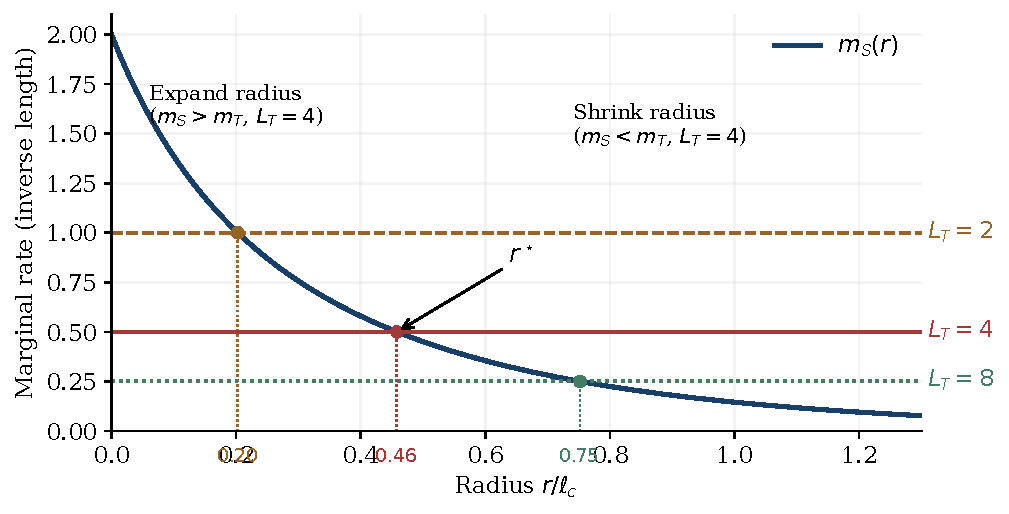
\includegraphics[width=.92\linewidth]{figures/marginal_balance.pdf}
\caption{Marginal balance in the canonical model with $\ell_c=1$ and
$\ell_s=0.5$. Increasing $L_T=vT$ lowers $m_T=2/L_T$ and moves the crossing
with $m_S$ outward. For the middle curve ($L_T=4$), regret falls to the left
of the crossing and rises to its right. This is an illustration of the
analytical rates, not an additional numerical experiment.}
\label{fig:marginal-balance}
\end{figure}

The resulting design principle is to expand information radius while the
marginal spatial value exceeds the marginal freshness loss, stopping at their
balance when the optimum is interior.

\subsection{Canonical Line Model and Closed-Form Radius}
\label{subsec:canonical_line_model}

We now derive the spatial omission function and the optimal radius from a
concrete stochastic field and decision model. Consider a dense one-dimensional network, represented by locations
$z\in\mathbb{R}$. This is also the continuum approximation of a sufficiently
long path graph away from its boundaries.


Let $\theta(z,t)$ be a zero-mean Gaussian field with covariance
\begin{equation}
    \mathbb{E}
    \left[
        \theta(z,t)\theta(z',s)
    \right]
    =
    \sigma^2
    \exp
    \left(
        -\frac{|z-z'|}{\ell_s}
    \right)
    \exp
    \left(
        -\frac{|t-s|}{T}
    \right).
    \label{eq:canonical_space_time_covariance}
\end{equation}
The parameter $\ell_s$ is the spatial correlation length, and $T$ is the
temporal coherence time.

Suppose the full-information decision at location $z$ is the exponentially
weighted spatial aggregate
\begin{equation}
    x^\star(z,t)
    =
    \int_{-\infty}^{\infty}
    w_{\ell_c}(u)
    \theta(z+u,t)\,du,
    \label{eq:canonical_target}
\end{equation}
where
\begin{equation}
    w_{\ell_c}(u)
    \triangleq
    \frac{1}{2\ell_c}
    \exp
    \left(
        -\frac{|u|}{\ell_c}
    \right).
    \label{eq:exponential_decision_kernel}
\end{equation}

$w_{\ell_c}$ is the Laplace (two-sided exponential) density: it integrates to one, so $x^\star(z,t)$ is a weighted average of the field around $z$. The weight falls by a factor $e$ for each $\ell_c$ of distance, and the average distance $\mathbb E|u|$ under this weight equals $\ell_c$.

The decision-relevance length $\ell_c$ controls how broadly remote states
influence the desired local action.

For example, \eqref{eq:canonical_target} is generated pointwise by the
quadratic tracking-loss density
\begin{equation}
    f_z(x,\theta)
    =
    \frac{q}{2}
    \left[
        x(z)-x^\star(z,\theta)
    \right]^2,
    \qquad q>0.
    \label{eq:canonical_tracking_cost}
\end{equation}
In this canonical model, all nonlocal dependence enters through the \emph{target}, not through interaction between actions. The pointwise cost \eqref{eq:canonical_tracking_cost} has no cross terms between $x(z)$ and $x(z')$; this is the continuum analogue of a diagonal $Q=qI$. The linear term is $b(\theta)(z)=q\,x^\star(z,\theta)$, which depends on the field over a range of order $\ell_c$. Each location's optimal policy is therefore just its own conditional mean, $\mathbb E[x^\star(z,t)\mid\text{information at }z]$.

On the infinite line, a positive homogeneous regret density gives infinite total expected regret. We therefore measure regret \emph{per unit length}, which by stationarity equals the expected pointwise loss at any single location $z$. With this convention, $R_\infty=(q/2)\operatorname{Var}(x^\star(z,t))$. Direct action coupling would change the form of $\eta_S(r)$, but not the composition law \eqref{eq:regret_composition_unnormalized} or Proposition~\ref{thm:marginal_balance}.

At zero delay, the radius-$r$ observation at location $z$ is
\begin{equation}
    \mathcal{O}_r(z,t)
    \triangleq
    \sigma
    \left(
        \theta(z+u,t):
        |u|\le r
    \right).
    \label{eq:canonical_radius_observation}
\end{equation}

Formally, the observation $\sigma$-algebra \eqref{eq:canonical_radius_observation} is generated by uncountably many values. The exponential-covariance field admits a continuous version, which we use. Consequently, this $\sigma$-algebra is generated equally well by the values on a countable dense subset of the observed interval (including the center for a radius-zero snapshot), up to completion by probability-zero events. Conditional expectations are well defined in either formulation.

\begin{lemma}[Exponential omission by self-similarity]
\label{prop:canonical_eta_S}
For the field \eqref{eq:canonical_space_time_covariance}, decision
\eqref{eq:canonical_target}, and observation
\eqref{eq:canonical_radius_observation}, the normalized zero-delay spatial
omission error is
\begin{equation}
    \boxed{
    \eta_S(r)
    =
    \frac{
        \ell_c
    }{
        \ell_c+2\ell_s
    }
    \exp
    \left(
        -\frac{2r}{\ell_c}
    \right).
    }
    \label{eq:canonical_eta_S}
\end{equation}
In particular,
\begin{equation}
    \eta_0
    =
    \eta_S(0)
    =
    \frac{
        \ell_c
    }{
        \ell_c+2\ell_s
    }.
    \label{eq:canonical_eta_zero}
\end{equation}
\end{lemma}

\begin{proof}
By spatial stationarity, take $z=0$ and suppress the time argument. Write $\beta_c\triangleq1/\ell_c$ and $\beta_s\triangleq1/\ell_s$ for the inverse lengths, so $w(u)=\tfrac{\beta_c}{2}e^{-\beta_c|u|}$ and $\operatorname{Cov}(\theta(u),\theta(u'))=\sigma^2e^{-\beta_s|u-u'|}$.

\textbf{Step 0 (omission is a variance ratio).} With $Q=qI$ the optimal policy given $\mathcal O_r$ is $\mathbb E[x^\star(0)\mid\mathcal O_r]$. Its expected loss is $\tfrac q2\,\mathbb E\big[\operatorname{Var}(x^\star(0)\mid\mathcal O_r)\big]$. For a Gaussian field the conditional variance is a deterministic number: it does not depend on the observed values (Appendix~\ref{app:toolkit-3}). Since $R_\infty=\tfrac q2\operatorname{Var}(x^\star(0))$,

\[
\eta_S(r)=\frac{\operatorname{Var}(x^\star(0)\mid\mathcal O_r)}{\operatorname{Var}(x^\star(0))}.
\]


\textbf{Step 1 (split into observed middle and two tails).} Write $x^\star(0)=M_r+T_r^++T_r^-$, where

\[
M_r=\int_{-r}^{r}w(u)\theta(u)\,du,\qquad T_r^+=\int_r^\infty w(u)\theta(u)\,du,\qquad T_r^-=\int_{-\infty}^{-r}w(u)\theta(u)\,du .
\]

The middle $M_r$ is computed from observed values, so it contributes no conditional variance.

\textbf{Step 2 (rewrite the right tail).} Substituting $u=r+s$,

\[
T_r^+=\frac{\beta_c}{2}e^{-\beta_c r}\,Y_r,\qquad Y_r\triangleq\int_0^\infty e^{-\beta_c s}\,\theta(r+s)\,ds .
\]


\textbf{Step 3 (spatial Markov property).} By Section~\ref{sec:spatiotemporal_predictability}, the field is Markov in $z$. Given the observed segment $[-r,r]$, the right tail $\{\theta(u):u>r\}$ and the left tail $\{\theta(u):u<-r\}$ are conditionally independent, and each depends on the segment only through its adjacent endpoint $\theta(r)$ or $\theta(-r)$. Therefore

\[
\operatorname{Var}(T_r^+\mid\mathcal O_r)=\operatorname{Var}(T_r^+\mid\theta(r)),\qquad \operatorname{Var}(T_r^-\mid\mathcal O_r)=\operatorname{Var}(T_r^-\mid\theta(-r)),\qquad \operatorname{Cov}(T_r^+,T_r^-\mid\mathcal O_r)=0 .
\]


\textbf{Step 4 (the tail variance does not depend on $r$).} Define $C\triangleq\operatorname{Var}(Y_0\mid\theta(0))$. Shifting the field by $r$ does not change its law, so $\operatorname{Var}(Y_r\mid\theta(r))=C$ for every $r$. By reflection symmetry (the covariance depends only on $|u-u'|$), the left tail gives the same value. Hence

\[
\operatorname{Var}(x^\star(0)\mid\mathcal O_r)=2\Big(\frac{\beta_c}{2}\Big)^2e^{-2\beta_c r}\,C=\frac{\beta_c^2}{2}e^{-2\beta_c r}\,C .
\]

At $r=0$ the same argument applies with $\mathcal O_0=\sigma(\theta(0))$ and $M_0=0$, giving $\operatorname{Var}(x^\star(0)\mid\theta(0))=\tfrac{\beta_c^2}{2}C$. Dividing, $\eta_S(r)=\eta_S(0)\,e^{-2\beta_c r}=\eta_S(0)\,e^{-2r/\ell_c}$. The unknown constant $C$ cancels, so it never has to be computed.

\textbf{Step 5 (the constant $\eta_S(0)$).} Conditioning on the single Gaussian variable $\theta(0)$ gives $\operatorname{Var}(x^\star(0)\mid\theta(0))=\operatorname{Var}(x^\star(0))\big(1-\operatorname{Corr}(x^\star(0),\theta(0))^2\big)$ (Appendix~\ref{app:toolkit-3}), so $\eta_S(0)=1-\operatorname{Corr}^2$. Two moments are needed.

\emph{Covariance with the local value:}

\[
\operatorname{Cov}(x^\star(0),\theta(0))=\int_{\mathbb R}w(u)\,\sigma^2e^{-\beta_s|u|}\,du=\frac{\sigma^2\beta_c}{2}\int_{\mathbb R}e^{-(\beta_c+\beta_s)|u|}\,du=\frac{\sigma^2\beta_c}{\beta_c+\beta_s}.
\]


\emph{Variance of the target:} $\operatorname{Var}(x^\star(0))=\frac{\sigma^2\beta_c^2}{4}\,I$, where $I\triangleq\iint e^{-\beta_c(|u|+|v|)-\beta_s|u-v|}\,du\,dv$.

To evaluate $I$, define the inner integral $h(u)\triangleq\int_{\mathbb R}e^{-\beta_c|v|}e^{-\beta_s|u-v|}\,dv$. Then $h$ is even, so $I=2\int_0^\infty e^{-\beta_c u}h(u)\,du$. For $u\ge0$, split the $v$-integral at $0$ and $u$:

\[
h(u)=\underbrace{\frac{e^{-\beta_s u}}{\beta_c+\beta_s}}_{v<0}+\underbrace{\frac{e^{-\beta_c u}-e^{-\beta_s u}}{\beta_s-\beta_c}}_{0\le v\le u}+\underbrace{\frac{e^{-\beta_c u}}{\beta_c+\beta_s}}_{v>u}.
\]

(The middle term is read as $u\,e^{-\beta_c u}$ when $\beta_s=\beta_c$.) Multiply by $e^{-\beta_c u}$ and integrate over $u\ge0$ term by term:

\[
\frac{1}{(\beta_c+\beta_s)^2},\qquad \frac{1}{\beta_s-\beta_c}\Big(\frac{1}{2\beta_c}-\frac{1}{\beta_c+\beta_s}\Big)=\frac{1}{2\beta_c(\beta_c+\beta_s)},\qquad \frac{1}{2\beta_c(\beta_c+\beta_s)} .
\]

Summing and doubling,

\begin{equation}
I=2\left[\frac{1}{(\beta_c+\beta_s)^2}+\frac{1}{\beta_c(\beta_c+\beta_s)}\right]=\frac{2(2\beta_c+\beta_s)}{\beta_c(\beta_c+\beta_s)^2},\qquad \operatorname{Var}(x^\star(0))=\frac{\sigma^2\beta_c(2\beta_c+\beta_s)}{2(\beta_c+\beta_s)^2}.
\label{eq:unconditional_target_variance}
\end{equation}


\emph{Combine.} With $\operatorname{Var}(\theta(0))=\sigma^2$,

\[
\operatorname{Corr}^2=\frac{\big(\sigma^2\beta_c/(\beta_c+\beta_s)\big)^2}{\sigma^2\cdot\sigma^2\beta_c(2\beta_c+\beta_s)/\big(2(\beta_c+\beta_s)^2\big)}=\frac{2\beta_c}{2\beta_c+\beta_s},\qquad \eta_S(0)=\frac{\beta_s}{2\beta_c+\beta_s}=\frac{\ell_c}{\ell_c+2\ell_s}.
\]
\end{proof}

Assume information propagates at effective speed $v>0$, so
\begin{equation}
    \tau(r)=r/v,
    \label{eq:linear_propagation_delay}
\end{equation}
and define the temporal propagation length
\begin{equation}
    L_T\triangleq vT.
    \label{eq:temporal_propagation_length}
\end{equation}
This is the distance information can travel during one coherence time.
We write $[z]_+\triangleq\max\{z,0\}$.

\begin{theorem}[Optimal synchronized-snapshot radius in the canonical model]
\label{thm:canonical_optimal_radius}
Suppose the state field obeys
\eqref{eq:canonical_space_time_covariance}, the full-information decision is
given by \eqref{eq:canonical_target}, the loss is
\eqref{eq:canonical_tracking_cost}, and the latency is
\eqref{eq:linear_propagation_delay}. Then the unique optimal radius on
the infinite line satisfies the dimensionless law
\begin{equation}
    \boxed{
    \frac{r^\star}{\ell_c}
    =
    \frac{1}{2}
    \left[
        \log
        \left(
            \frac{
                1+L_T/\ell_c
            }{
                1+2\ell_s/\ell_c
            }
        \right)
    \right]_+.
    }
    \label{eq:canonical_dimensionless_law}
\end{equation}
Equivalently,
\begin{equation}
    \boxed{
    r^\star
    =
    \frac{\ell_c}{2}
    \left[
        \log
        \left(
            \frac{
                \ell_c+L_T
            }{
                \ell_c+2\ell_s
            }
        \right)
    \right]_+.
    }
    \label{eq:canonical_optimal_radius}
\end{equation}

The optimal radius is strictly positive if and only if
\begin{equation}
    \boxed{
    L_T>2\ell_s.
    }
    \label{eq:positive_radius_condition}
\end{equation}
Within the interior regime, $r^\star$:

\begin{enumerate}
    \item increases with the temporal coherence time $T$;
    \item increases with the information-propagation speed $v$;
    \item decreases with the spatial correlation length $\ell_s$; and
    \item increases with the decision-relevance length $\ell_c$.
\end{enumerate}
\end{theorem}

\begin{proof}
With $\tau(r)=r/v$ we have $2\tau(r)/T=2r/L_T$. Substituting this and
$\eta_S(r)=\eta_0e^{-2r/\ell_c}$ into \eqref{eq:radius_regret_master} gives
\[
\frac{R(r)}{R_\infty}
=1-e^{-2r/L_T}(1-\eta_0e^{-2r/\ell_c})=1-g(r),
\]
so minimizing $R$ is the same as maximizing $g$.

For any omission law $\eta_S(r)=\eta_0e^{-2r/\ell_c}$ with
$0<\eta_0<1$, minimizing \eqref{eq:radius_regret_master} under linear delay
is equivalent to maximizing
\[
    g(r)=e^{-2r/L_T}-\eta_0e^{-2r(1/L_T+1/\ell_c)}.
\]
Differentiation gives
\[
    g'(r)=2e^{-2r/L_T}
    \left[\eta_0\left(\frac{1}{L_T}+\frac{1}{\ell_c}\right)
    e^{-2r/\ell_c}-\frac{1}{L_T}\right].
\]
The bracket is strictly decreasing and has a negative limit, so $g'$ changes
sign at most once, from positive to negative. If its value at zero is
nonpositive, radius zero is the unique optimum; otherwise the unique
stationary point is the optimum. Setting the bracket in $g'(r)$ to zero gives
\[
 e^{2r/\ell_c}=\eta_0 L_T\left(\frac1{L_T}+\frac1{\ell_c}\right)
 =\eta_0\left(1+\frac{L_T}{\ell_c}\right).
\]
Taking logarithms gives the stationary point below. It is positive exactly
when $\eta_0(1+L_T/\ell_c)>1$. Substituting
$\eta_0=\ell_c/(\ell_c+2\ell_s)$ makes this product
$(\ell_c+L_T)/(\ell_c+2\ell_s)$, which exceeds one exactly when
$L_T>2\ell_s$, as in \eqref{eq:positive_radius_condition}.
Thus the general exponential law gives
\begin{equation}
    r^\star=\frac{\ell_c}{2}
       \left[\log\!\left(\eta_0\left(1+\frac{L_T}{\ell_c}\right)\right)\right]_+,
    \label{eq:generic_exponential_rstar}
\end{equation}
and a maximum allowed radius $D$ gives
\begin{equation}
    r_D^\star=\min\{D,r^\star\}.
    \label{eq:capped_generic_rstar}
\end{equation}
Substituting $\eta_0=\ell_c/(\ell_c+2\ell_s)$ gives
\eqref{eq:canonical_dimensionless_law}--\eqref{eq:positive_radius_condition}.
The cap $D$ limits how far each agent may look, but the environment remains an
infinite line. In particular $\eta_S(D)=\eta_0e^{-2D/\ell_c}>0$. Unlike the
finite-graph endpoint $r=\operatorname{diam}(G)$, the capped radius still omits
decision-relevant state (compare Fig.~\ref{fig:radius-regret}, right panel).

In the positive-radius regime,
$\partial r^\star/\partial L_T=\ell_c/[2(\ell_c+L_T)]>0$ and
$\partial r^\star/\partial\ell_s=-\ell_c/(\ell_c+2\ell_s)<0$.
Since $L_T=vT$, these establish the first three comparative statics.
Finally, monotonicity in $\ell_c$ is not immediate from
\eqref{eq:canonical_optimal_radius}, because $\ell_c$ appears both as the
prefactor and inside the logarithm. Write the difference of logarithms as
\[
\log(\ell_c+L_T)-\log(\ell_c+2\ell_s)
=\int_{2\ell_s}^{L_T}\frac{ds}{\ell_c+s}.
\]
When $L_T>2\ell_s$ this gives
\begin{equation}
    r^\star
    =
    \frac{1}{2}
    \int_{2\ell_s}^{L_T}
    \frac{
        \ell_c
    }{
        \ell_c+s
    }
    ds.
    \label{eq:rstar_integral_representation}
\end{equation}
The integrand $\ell_c/(\ell_c+s)=1-s/(\ell_c+s)$ is strictly increasing
in $\ell_c$ for every $s>0$, proving that
$r^\star$ increases with the range over which remote state affects the
desired decision.
\end{proof}

Theorem~\ref{thm:canonical_optimal_radius} identifies three physical length
scales:

\begin{equation}
    \boxed{
    \underbrace{\ell_s}_{\text{spatial correlation}}
    \qquad
    \underbrace{\ell_c}_{\text{decision relevance}}
    \qquad
    \underbrace{L_T=vT}_{\text{temporal propagation}}.
    }
    \label{eq:three_length_scales}
\end{equation}

Three consequences clarify how these lengths determine the optimum.

\textbf{(1) The threshold does not depend on $\ell_c$.} At radius zero, using $\eta_S'(r)=-(2/\ell_c)\eta_S(r)$ and $\eta_0/(1-\eta_0)=\ell_c/(2\ell_s)$,

\[
m_S(0)=\frac{2}{\ell_c}\cdot\frac{\eta_0}{1-\eta_0}=\frac{1}{\ell_s},\qquad m_T=\frac{2}{L_T}.
\]

The first increment of radius pays off exactly when $1/\ell_s>2/L_T$, that is, $L_T>2\ell_s$. The decision range $\ell_c$ cancels because it has two offsetting effects at $r=0$. A longer decision range makes the local observation less complete (larger $\eta_0$), which raises the value of looking farther. But it also makes omission decay more slowly with radius (rate $2/\ell_c$), which lowers the value of each extra unit of radius.

\textbf{(2) Long decision range}, $\ell_c\gg L_T,\ell_s$. In the positive-radius regime $L_T>2\ell_s$, using $\log\frac{1+a}{1+b}=\log(1+a)-\log(1+b)\approx a-b$ for small $a,b$,

\[
r^\star\approx\frac{\ell_c}{2}\Big(\frac{L_T}{\ell_c}-\frac{2\ell_s}{\ell_c}\Big)=\frac{L_T-2\ell_s}{2},
\]

half the excess propagation length.

\textbf{(3) Short decision range}, $\ell_c\ll\ell_s,L_T$. Then $\ell_c+L_T\approx L_T$ and $\ell_c+2\ell_s\approx2\ell_s$, so $r^\star\approx(\ell_c/2)\log\big(L_T/(2\ell_s)\big)$ when $L_T>2\ell_s$, and $r^\star=0$ otherwise.

\textbf{Why does stronger spatial correlation shrink the optimal radius?} This can seem backwards: more correlation sounds like it should make neighbors more useful. But $\eta_0=\ell_c/(\ell_c+2\ell_s)$ falls as $\ell_s$ grows. When the field is smooth, the local value $\theta(z)$ already predicts the field well over the whole decision range, so little is left for a wider snapshot to add. Extra radius mostly reports values the agent could already have predicted. Its marginal value $m_S(r)=\frac{2}{\ell_c}\frac{\eta_S(r)}{1-\eta_S(r)}$ is therefore smaller at every radius, while its freshness cost $m_T$ is unchanged, and the balance point moves inward. Correlation makes neighbors informative, but it also makes them redundant with what the agent already knows.

On a finite graph, Theorem~\ref{thm:spatiotemporal_composition} and minimization
over integer radii remain exact, with the one-hop comparison
\eqref{eq:discrete_radius_improvement}--\eqref{eq:discrete_radius_log_improvement}
as the discrete form of marginal balance; Eq.~\eqref{eq:canonical_optimal_radius}
is the closed-form counterpart on the homogeneous line.





\section{Numerical Consistency Checks and Finite-Graph Illustrations}
\label{sec:numerical-evaluation}

This section checks the implementations against the closed-form predictions
and then shows how the same quantities behave on finite graphs.  Experiments 1 and 2
check temporal prediction and the fresh-local--stale-global endpoints;
Experiments 3 and 4 isolate and sweep the continuous radius tradeoff;
Experiment 5 separates state statistics from decision-relevant omission; and
Experiment 6 evaluates exact integer radii on several noncanonical graph
instances.

\subsection{Numerical Methodology and Synthetic Environments}
\label{subsec:numerical-methodology}

The numerical objects are architecture regrets, so each calculation uses the
same information structure as its analytical counterpart.  We work with an
exogenous common-rate Gaussian-affine environment: actions do not alter later
states.  For
$x^\star=K\theta+k_0$, with $K=Q^{-1}B$, we evaluate
\begin{equation*}
    R(\mathcal A)=\tfrac12
    \left\|x^\star-u_{\mathcal A}^\star\right\|_Q^2
\end{equation*}
from conditional covariance and, where appropriate, from independently
sampled quadratic losses.  The solvers respect the information structure: the
common delayed snapshot in Experiment 1 permits a joint conditional mean even
for non-diagonal $Q$; Experiment 2 uses the exact fresh-local rule; Experiments
3 and 4 evaluate the scalar composition; and Experiments 5 and 6 use $Q=I$ so
agentwise Gaussian conditional variances are exact.  Experiment 5 holds the
graph and covariance fixed while changing decision sensitivity.  The graph
covariances are scaled to average marginal variance one.

For an arbitrary graph, a convenient alternative is to define the covariance
spectrally through the graph Laplacian $L_G$. For example,
\begin{equation}
    \Sigma_S
    =
    \sigma^2
    \left(
        \kappa_s^2 I+L_G
    \right)^{-\nu},
    \qquad
    \kappa_s>0,\quad \nu>0,
    \label{eq:graph_spectral_covariance}
\end{equation}
is positive semidefinite and places more state energy in low graph-frequency
modes. Such constructions are closely related to graph signal smoothness and
Gaussian Markov random-field models
\cite{shuman2013emerging,lindgren2011explicit}.

Pointwise Monte Carlo means use 95\% normal confidence intervals.  The
Experiment 2 boundary intervals apply the delta method to the paired
fresh-local/open-loop regret means, so their uncertainty reflects that
the two regrets use the same draws.

Table~\ref{tab:numerical-parameters} summarizes the reference settings.  The
repository stores fixed configurations, processed tables, selected raw arrays,
and graph covariance/distance inputs where applicable, together with run
metadata and diagnostics; it is not a complete archive of every random draw.
The exact system construction, graph seeds, conditioning safeguards, boundary
conventions, radius grids, crossover estimator, and interval calculation are
specified in the reproduction documentation.  Robustness beyond the
common-rate Gaussian-affine model is discussed in
Section~\ref{sec:discussion_conclusions}.

\begin{table}[H]
\centering
\caption{Reference numerical settings. The shared-resource sweep fixes $q=1$;
graph covariances in Experiments 5--6 are scaled to average marginal variance
one. Quantities not being swept retain the experiment-specific values in the
configuration files.}
\label{tab:numerical-parameters}
\small
\begin{tabular}{llll}
\toprule
Experiment & principal sweep & fixed setting/size & evaluation \\
\midrule
1. Temporal pairs & $\tau/T\in[0,3]$ (25 points) & A--D; $n=8,20,50,32$ & $20{,}000$/point \\
2. Local--global & 9 $\gamma/q$ values in $[0,10]$ & $n=5,10,25,100$; $q=1$ & $30{,}000$/setting \\
3. Scalar radius & $r/\ell_c\in[0,2]$ (1,001 points) & 3 regimes; $D/\ell_c=2$ & $50{,}000$/point \\
4. Canonical map & $(vT/\ell_c,\ell_s/\ell_c)$; $72\times68$ & $r/\ell_c\in[0,4]$; $\Delta r=0.0016$ & direct scalar \\
5. Decision relevance & $\ell_c=0.7,2,6$ & 64-node ring; $T=6$ & $12{,}000$/check \\
6. General graphs & path, ring, grid, geometric & 64 nodes; $T=5$ & exact covariance \\
\bottomrule
\end{tabular}
\end{table}

\subsection{Temporal Scaling and the Local--Global Crossover}
\label{subsec:numerical-temporal-crossover}

The first two experiments test two different consequences of common-rate
temporal predictability: the exact stale-global law
\eqref{eq:OU_exact_regret}, and the endpoint crossover threshold
\eqref{eq:aggregate_rho_star}.

Experiment 1 asks whether the normalized regret of a delayed global snapshot
depends only on $\rho=\tau/T$, even when spatial covariance, objective
coupling, and the decision operator change.  We used the four systems in
Table~\ref{tab:numerical-parameters} and drew 20,000 exact stationary OU pairs
$(\theta_{t-\tau},\theta_t)$ at each of 25 values of $\rho$.  The first member
has covariance $\Sigma_S$ and the second is generated as
$e^{-\rho}\theta_{t-\tau}+(1-e^{-2\rho})^{1/2}\varepsilon$, with an
independent innovation $\varepsilon$ of covariance $\Sigma_S$.  For each pair,
the optimal delayed-snapshot action was evaluated with the known common-rate
coefficient and the quadratic loss was computed in the system's $Q$ metric.

Across the 100 system--parameter combinations, the Monte Carlo curves collapse
onto $1-e^{-2\tau/T}$ (Fig.~\ref{fig:temporal-scaling}).  The largest absolute
normalized deviation was $0.0155$ and the root-mean-square deviation was
$0.00471$.  This supports the exact temporal scaling for these stationary
common-rate pairs.

\begin{figure}[t]
\centering
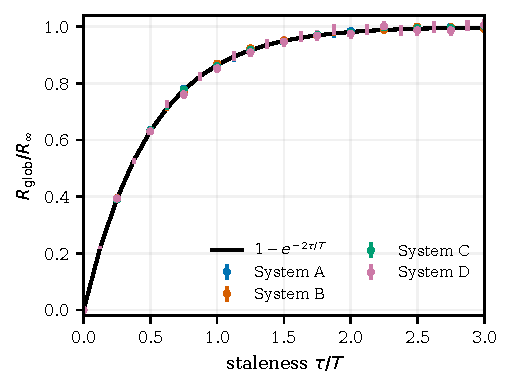
\includegraphics[width=0.82\linewidth]{figures/fig7_1_temporal_scaling.pdf}
\caption{Temporal scaling collapse from exact stationary OU pairs. Markers are
Monte Carlo estimates for four systems with different dimensions, spatial
covariances, objective matrices, and decision operators; bars are 95\%
confidence intervals. The solid curve is the exact law
$1-e^{-2\tau/T}$. Normalization by $R_\infty$ removes system-specific scale.}
\label{fig:temporal-scaling}
\end{figure}

Experiment 2 asks whether the finite-$n$ threshold in
Eq.~\eqref{eq:aggregate_rho_star} describes the point at which fresh local
information becomes preferable to a stale global snapshot.  We used the
shared-resource model
$Q=qI+\gamma\mathbf 1\mathbf 1^\top$, $q=1$, with independent OU
components.  For each of 36 $(n,\gamma/q)$ settings, the fresh-local and
open-loop regrets were evaluated on the same 30,000 current-state draws.  The
empirical boundary was then inferred by inserting these two estimates into
the OU temporal law,
\begin{equation*}
    \widehat\rho^\star
    =
    \frac12\log\left(
        \frac{\widehat R_\infty}
        {\widehat R_\infty-\widehat R_{\rm loc}}
    \right).
\end{equation*}
Accordingly, Fig.~\ref{fig:local-global-phase} reports the temporal-law boundary
inferred from paired local/open-loop losses.

The mean absolute boundary error was $0.00111$ and the maximum was $0.00557$.
Finite size matters most under strong coupling: at $n=5$ and $\gamma/q=10$,
the exact threshold is $0.109$ below the large-system limit.  As $n$ grows,
the inferred boundary approaches $\tfrac12\log(1+\gamma/q)$.  Stronger
decision coupling therefore makes older global information worth tolerating
in this independent-component model.

\begin{figure}[t]
\centering
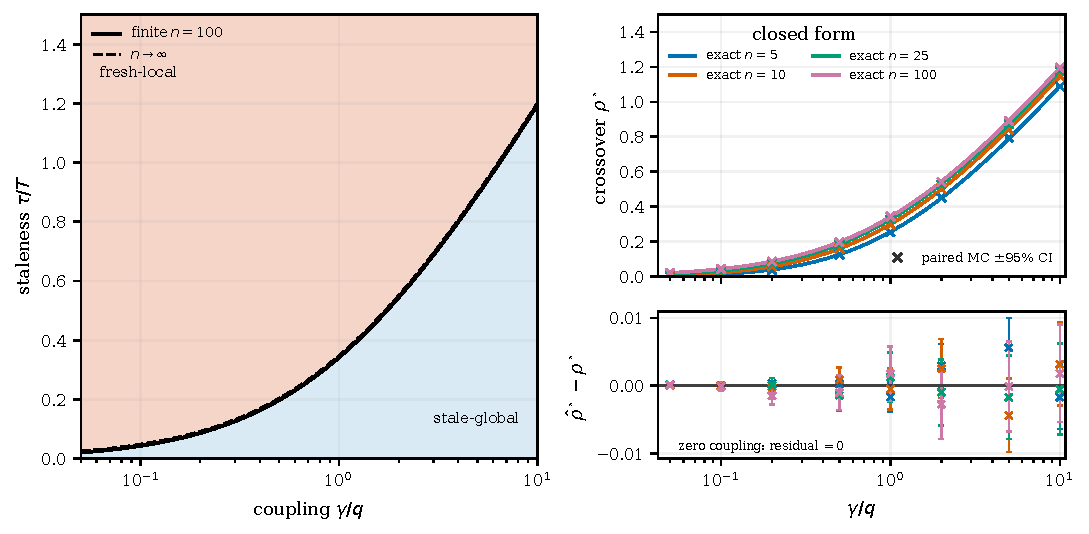
\includegraphics[width=0.98\linewidth]{figures/fig7_2_local_global_phase.pdf}
\caption{Fresh-local versus stale-global crossover. Left: the phase map uses the
exact finite-$n=100$ boundary (solid) and the large-$n$ limit (dashed),
Eqs.~\eqref{eq:aggregate_rho_star} and \eqref{eq:large_n_threshold}.
Upper right: exact theory curves and inferred Monte Carlo
boundaries (crosses) for four system sizes, with paired delta-method 95\%
intervals. Lower right: empirical minus theoretical boundary, on a scale that
reveals the sampling differences and their uncertainty.
The zero-coupling setting is evaluated at $\rho^\star=0$ but omitted from the
logarithmic positive-coupling axes.}
\label{fig:local-global-phase}
\end{figure}

\subsection{Emergence of an Optimal Coordination Radius}
\label{subsec:numerical-radius-curves}

Experiment 3 illustrates why expanding the information radius can help at
first and hurt later: reduced spatial omission competes with increasing
staleness.  We used
$\eta_S(r)=\eta_0e^{-2r/\ell_c}$ and $\tau(r)=r/v$ on
$0\le r\le D=2$, with local $(\eta_0,vT)=(0.25,0.2)$, interior
$(0.7,4)$, and maximum allowed radius $(0.9,100)$ regimes (all with
$\ell_c=1$). At each
radius, independent standard-normal draws were scaled by the two prescribed
component variances and added before squaring.  This is a scalar loss check:
no spatial field, graph, or neighborhood conditional distribution is sampled.

The grid minima were $0$, $0.626$, and $2$; the corresponding analytical
minima after imposing the cap were $0$, $0.62638$, and $2$.  At the interior
grid minimum, the marginal-slope gap was
\mbox{$|m_S(\hat r^\star)-m_T(\hat r^\star)|=4.77\times10^{-4}$}, and the largest
Monte Carlo deviation from the prescribed scalar curve was about $0.020$.
The maximum allowed radius case is not a global endpoint: its
unconstrained minimizer lies beyond $D$, while
$\eta_S(D)=\eta_0e^{-2D/\ell_c}>0$.  Thus the cap still omits
decision-relevant state.  The three curves distinguish immediate dominance of
staleness, an interior balance, and a benefit from expansion throughout the
allowed range.

\begin{figure}[t]
\centering
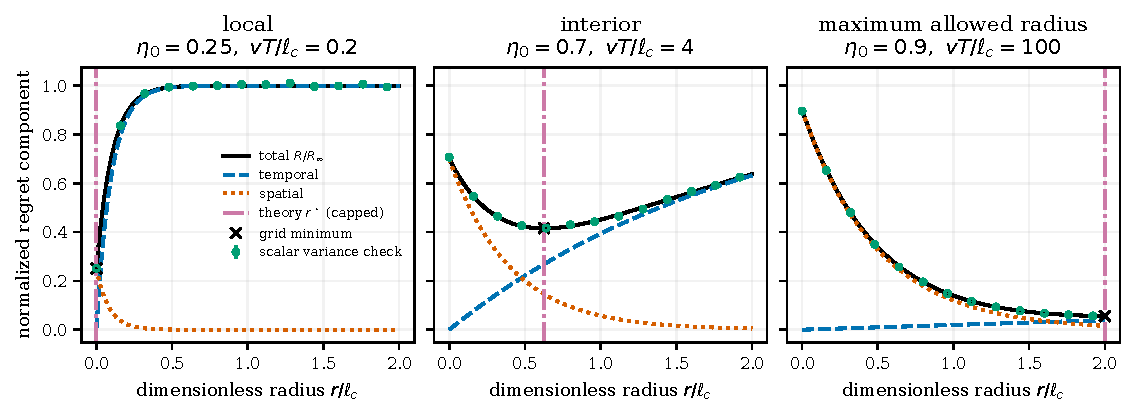
\includegraphics[width=\linewidth]{figures/fig7_3_radius_regret.pdf}
\caption{Emergence of local, interior, and maximum allowed radius optima under
$\eta_S(r)=\eta_0e^{-2r/\ell_c}$ and $\tau(r)=r/v$. Curves show total regret
and its temporal and residual-spatial terms from Eq.~\eqref{eq:R_decomposition};
open markers with 95\% intervals are independent scalar-innovation estimates.
Dash-dotted lines and crosses mark the analytical constrained and grid
minimizers. At the maximum allowed radius, positive omission remains:
$\eta_S(D)>0$.}
\label{fig:radius-regret}
\end{figure}

\subsection{Scaling Laws and Regime Map}
\label{subsec:numerical-radius-phase}

Experiment 4 asks whether the canonical closed form predicts both the
zero-radius region and the interior radius over a two-parameter sweep, rather
than only at selected examples.  We swept 4,896 points over
$vT/\ell_c\in[0.1,20]$ and $\ell_s/\ell_c\in[0.05,5]$, using $\ell_c=1$
as the unit of length. Independently of the closed form, every point was minimized by direct scalar evaluation of
Eq.~\eqref{eq:regret_composition_normalized} on the same fixed grid
$r_j=0.0016j$, $j=0,\ldots,2500$, so $r\in[0,4]$ for every parameter pair.
No covariance simulation or adaptive radius range was used.  Separate
one-dimensional sweeps tested the four comparative statics.

The gray region in Fig.~\ref{fig:radius-phase} selects fresh local information;
above the threshold $vT=2\ell_s$, positive scope becomes worthwhile.
Moving upward increases the distance information can travel within a coherence
time and raises the preferred radius. Moving right increases spatial
correlation, making remote observations more redundant and lowering the
preferred radius. The slices show these changes as ordinary radius curves.
The mean absolute grid-versus-closed-form error was
$2.25\times10^{-4}$ and the maximum was $8.00\times10^{-4}$, below the
$0.0016$ grid step.  Ordinary grid error occurs throughout the positive-radius
interior because the minimizer is discretized; it is not confined to the
threshold.  There were five zero/positive classification disagreements, all
adjacent to the threshold where the continuous optimum fell below the first
positive grid point.  The one-dimensional sweeps were monotone in all four
predicted directions: $r^\star$ increased with $T$, $v$, and $\ell_c$, and
decreased with $\ell_s$.  This validates the scalar search and canonical
scaling within the stated range.

\begin{figure}[t]
\centering
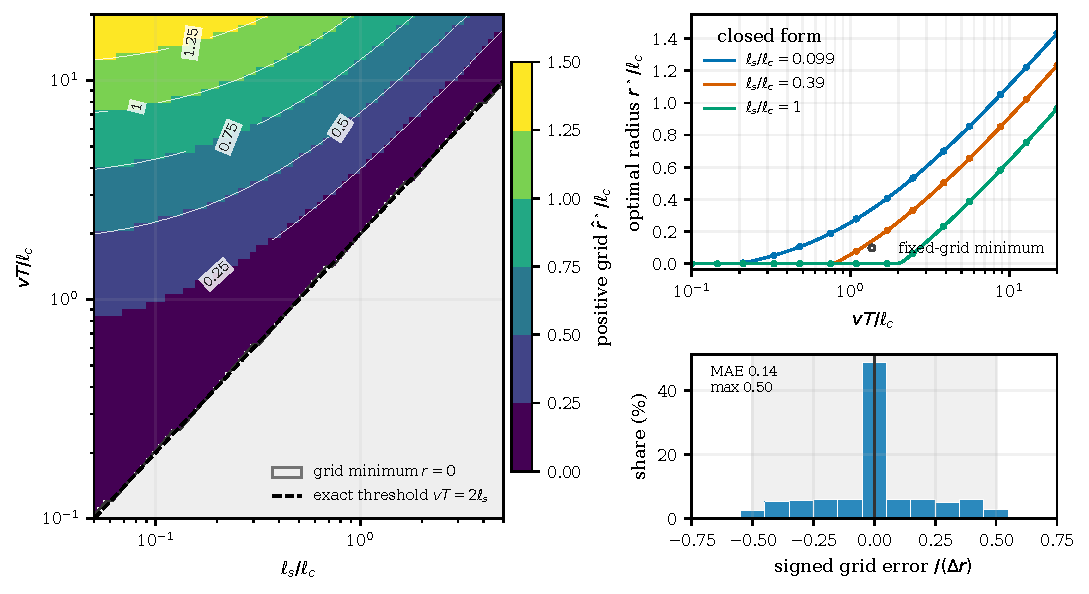
\includegraphics[width=0.98\linewidth]{figures/fig7_4_radius_phase.pdf}
\caption{Dimensionless optimal-radius law from direct scalar minimization. Left:
the numerical map, with the numerical zero-radius region shown in gray and the
dashed curve marking the theoretical transition $vT=2\ell_s$. Upper right:
selected $\ell_s/\ell_c$ slices comparing grid minimizers with the closed form
in Eq.~\eqref{eq:canonical_dimensionless_law}. Lower right: the histogram of
$(\hat r^\star-r^\star)/\Delta r$ over all 4,896 points; its zero spike
includes local-regime points and the remaining grid errors are of order a
half-step.}
\label{fig:radius-phase}
\end{figure}

\subsection{State Predictability versus Decision-Relevant Predictability}
\label{subsec:numerical-decision-relevance}

Experiment 5 asks whether the architecture depends on which state modes affect
the decision, rather than only on raw state correlation.  We held a 64-node
ring, its Laplacian covariance, $T=6$, and the latency law (0.12 time units per
hop) fixed, and changed only the decision-sensitivity operator
$K_{ij}=e^{-d_G(i,j)/\ell_c}/\|e^{-d_G(i,\cdot)/\ell_c}\|_2$, using
$\ell_c\in\{0.7,2,6\}$ and $Q=I$.  Exact Gaussian conditioning gives the
decision-weighted omission $\eta_S(r)$ at every graph radius.  The raw
state-correlation statistic was computed separately from the fixed covariance;
it is not the same quantity as $\eta_S(r)$.  Each curve is normalized by its
own $R_\infty=\tfrac12\operatorname{tr}(K\Sigma_S K^\top)$, so normalized
regrets compare unexplained fractions rather than equal absolute cost scales.

Increasing $\ell_c$ from $0.7$ to $2$ to $6$ increased $\eta_S(0)$ from
$0.0460$ to $0.258$ to $0.572$ and moved the discrete optimum from 1 to 2 to
5 hops, even though the raw state correlation was identical.  Independent
12,000-sample conditioning checks differed from the exact omission by at most
$2.39\times10^{-3}$ (the largest pointwise standard error was
$3.20\times10^{-3}$).  Thus changing only decision sensitivity in a fixed
environment produced substantially different preferred architectures.

\begin{figure}[t]
\centering
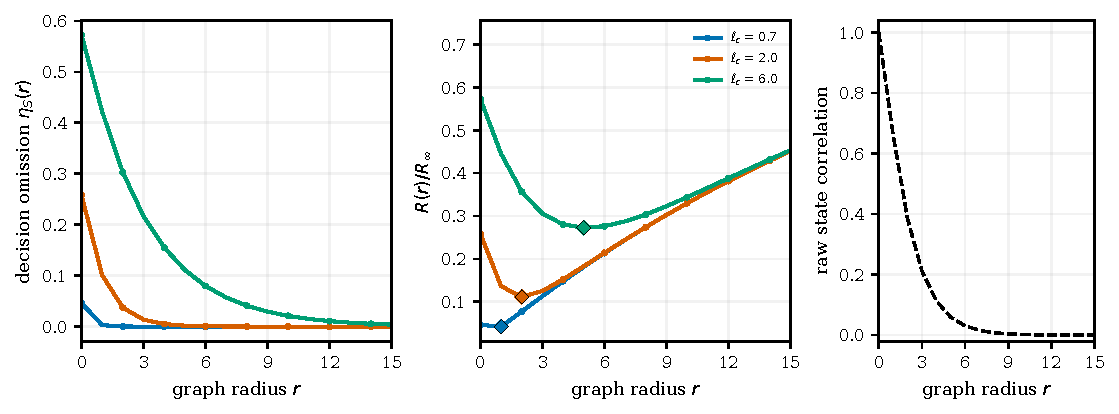
\includegraphics[width=0.94\linewidth]{figures/fig7_5_decision_relevance.pdf}
\caption{Decision relevance with the graph and state covariance held fixed.
The decision-weighted omission and normalized composed regret are shown for
three row-$\ell_2$-normalized operators with $Q=I$.  Raw state correlation is
shown in a separate context panel and is identical across operators; it is
not an omission estimate.  Each regret is normalized by its operator-specific
$R_\infty$, and the minimizing integer radius is marked.  Changing only the
decision-relevance range moves the optimum from 1 to 5 hops.}
\label{fig:decision-relevance}
\end{figure}

\subsection{Finite Graphs beyond the Canonical Geometry}
\label{subsec:numerical-general-graphs}

Experiment 6 asks whether the conditional-variance construction and discrete
radius comparison remain usable when the geometry is not the homogeneous line
assumed by the canonical formula.  We considered one 64-node graph of each of
a path, ring, two-dimensional grid, and random geometric type; the geometric
graph uses the fixed configured seed.  For each instance we formed the covariance \eqref{eq:graph_spectral_covariance},
scaled it to average marginal variance one, and computed every $\eta_S(r)$
directly from the Gaussian conditional
covariance of the desired action given the radius-$r$ neighborhood.  The
reference setting uses $Q=I$, $T=5$, $\ell_c=2$, and latency $0.12$ per hop.
No exponential omission fit or canonical line formula was used, and no graph
ensemble average was taken.

Under the reference setting, Fig.~\ref{fig:general-graphs} gives exact integer
optima of 2, 2, 3, and 2 hops for the path, ring, grid, and geometric instance,
respectively.  In these four sampled instances, increasing $T$ over the
configured values $1.5,2.5,4,6,9,14$ changed the optimum from 1 to 3 hops on
the path and ring, from 1 to 4 on the grid, and from 1 to 3 on the geometric
graph.  The sampled $\ell_c$ sweep from $0.7$ to $6$ moved the optima from
$(0,0,1,1)$ to $(5,5,5,3)$ in the same graph order. Increasing per-hop latency
weakly decreased the optimum, as did decreasing $\kappa_s$, which increases
spatial smoothness after variance normalization. These comparative statics
describe the four specified graph instances. Since radii are integer-valued,
the appropriate comparison is the one-hop regret difference in
Eq.~\eqref{eq:discrete_radius_improvement}. For example, the geometric graph's
three-hop regret exceeds its two-hop minimum by only $0.00362R_\infty$;
the archived neighbor differences quantify such shallow minima.

\begin{figure}[p]
\centering
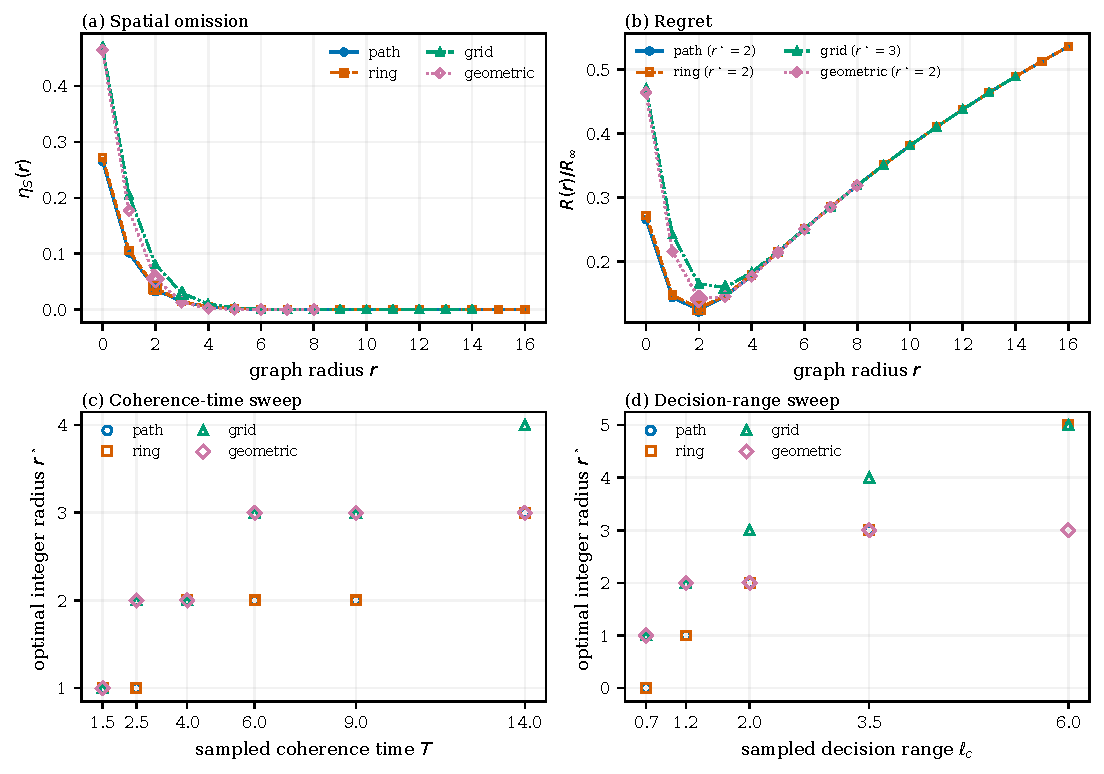
\includegraphics[width=\linewidth]{figures/fig7_6_general_graphs.pdf}
\caption{Finite noncanonical graphs. Top: $\eta_S(r)$ computed from exact
Gaussian conditional covariances and the resulting regret under one common
normalized setting; lines join integer-radius evaluations. Bottom: exact
integer optima at the sampled coherence times and decision ranges; no
transition locations between those settings are inferred. Distinct marker
shapes identify coincident graph results. The canonical line closed form is
not used.}
\label{fig:general-graphs}
\end{figure}
\clearpage

\section{Related Work}
\label{sec:related_work}

We organize the closest literatures around three distinctions: iterative
computation versus information architecture, controlled dynamics versus an
exogenous environment, and age-based freshness versus decision-relevant value.
These distinctions frame the more specific connections developed below.

\subsection{Static Team Decision Theory}
\label{subsec:related_static}

Radner established foundational optimality conditions for static teams, in which decision makers share a common objective but act on different information \cite{radner1962team}. Under appropriate convexity and regularity conditions, the resulting stationarity conditions are sufficient for global team optimality; in the quadratic Gaussian specialization, the optimal decision rules are affine \cite{radner1962team,marschak1972economic}. In the deterministic-Hessian quadratic model used here, these fixed-information optimality conditions admit the equivalent Hilbert-space formulation developed in Section~\ref{subsec:projection}: for a fixed information architecture $\mathcal A$, the team-optimal policy is the $Q$-orthogonal projection of the full-information action onto the closed subspace $\mathcal S(\mathcal A)$ of implementable policies. This projection identity specializes the classical static-team framework to our quadratic model; Radner's theorem is not stated in this literal form. Krainak, Speyer, and Marcus subsequently relaxed the sufficient conditions associated with Radner's stationarity result and extended the theory to an exponential-quadratic criterion with jointly Gaussian state and observations \cite{krainak1982staticI}. In a companion paper, they formulated affine linear-quadratic-Gaussian and linear-exponential-Gaussian team problems as constrained parameter optimizations and represented optimal team gains as projections of the corresponding centralized gains \cite{krainak1982staticII}.

Classical team theory also treated information itself as an organizational design object. Marschak and Radner analyzed the value of information, delayed information and the tradeoff between timeliness and completeness, and formulated team organization in terms of optimal networks \cite{marschak1972economic}. More recently, Summers, Li, and Kamgarpour formulated information-structure design as the selection of additional measurements or communication links jointly with the corresponding team decision strategies \cite{summers2017information}. Afshari and Mahajan characterized quadratic Gaussian static teams whose observations decompose into information common to all agents and agent-specific local information \cite{afshari2017static}. They subsequently applied this decomposition to team-optimal decentralized filtering over communication graphs with delayed information sharing, where sufficiently old measurements constitute common information while more recent measurements remain local \cite{afshari2018team}. Rusmevichientong and Van Roy studied large teams in which each agent observes the local cost structure only within a graph radius, using centralized performance as a benchmark \cite{rusmevichientong2003decentralized}. Gamarnik, Goldberg, and Weber studied decentralized decisions based on local information in random decision networks and related their near-optimality to a correlation-decay, or long-range-independence, property \cite{gamarnik2014correlation}.

Relative to these works, the distinctive object studied here is a structured family of information architectures in which spatial scope and temporal freshness are coupled through the scope--latency relation $\tau(r)$. Each spatial scope induces an acquisition delay, and the resulting architecture is valued through its prediction error for the full-information decision. This coupling yields the freshness--locality crossover and coordination-scale laws developed in Sections~\ref{sec:fresh_local_global} and \ref{sec:optimal_coordination_scale}.

\subsection{Distributed Optimization, Communication Constraints, and Scope}
\label{subsec:related_distributed_control}

Distributed optimization studies how agents compute a common solution using local computation and message exchange. Classical asynchronous gradient methods allow delayed interprocessor communication while retaining convergence guarantees under suitable boundedness conditions \cite{tsitsiklis1986distributed}, while distributed subgradient methods establish convergence when agents exchange information locally over time-varying network topologies \cite{nedic2009distributed}. In these canonical formulations, the communication process constrains an iterative computation of an optimizer. Our setting separates that computational question from information architecture: the full-information decision at each epoch is the benchmark, and the object of design is the information available when that decision must be made.

Networked and decentralized control place communication restrictions directly
in the feedback loop, including sampling, packet loss, communication topology,
and delay \cite{hespanha2007survey}. For spatially invariant plants, early work
showed that optimal controllers can exhibit inherent spatial localization
\cite{bamieh2002spatial}, while subsequent work imposed explicit finite-speed
communication structure. Arbelaiz, Bamieh, Hosoi, and Jadbabaie characterize
the spatial decay of optimal estimator gains, using the decay rate as a proxy
for the distance over which measurements are useful in a spatially distributed
dynamic estimation problem \cite{arbelaiz2025estimation}. Voulgaris, Bianchini, and Bamieh studied $H_2$ control
under delayed communication requirements \cite{voulgaris2003optimal}; Bamieh
and Voulgaris formulated distance-dependent information propagation through
funnel causality \cite{bamieh2005convex}; and Fardad and Jovanovi\'c developed
state-space models for distributed controllers with finite communication speed
\cite{fardad2011finite}. These works are important antecedents to our use of
spatial scope and propagation time, but they optimize dynamic feedback for
controlled plants rather than information-constrained stage decisions in an
exogenous environment.

Communication structure has also been treated as a design variable. Langbort
and Gupta study interconnection topology when communication is assigned a
topology-dependent cost \cite{langbort2009minimal}, and Matni co-designs
communication-delay structure and $H_2$ control using regularization
\cite{matni2017communication}. In wireless consensus, Vanka, Gupta, and Haenggi
explicitly trade communication radius against interference-induced delay
and show that the preferred connectivity depends on network geometry
\cite{vanka2010power}. Most directly, Ballotta, Jovanovi\'c, and Schenato
parameterize control architectures by communication scope: each agent receives
measurements from nodes within a chosen number of communication hops, with an
architecture-dependent delay that increases with that scope. After optimizing
the feedback gains for each scope, they show that sparse architectures can
outperform all-to-all feedback \cite{ballotta2023latency}. Ballotta and Gupta
obtain an analogous conclusion when maximizing consensus convergence speed
under hop-dependent communication delay \cite{ballotta2023sparser}. These
results establish that scope-dependent delay can itself induce a sparse or
intermediate optimal control architecture.

Our setting differs in the decision problem: an exogenous-state static team,
with the current full-information action as the benchmark and an architecture
valued by the prediction error it induces for that action. This yields the
decision-relevant spatial omission function $\eta_S(r)$, temporal
unpredictability $\eta_T(\tau)$, their exact common-rate composition law, and
the fresh-local versus stale-global and coordination-radius laws derived above.
Ballotta, Arbelaiz, Gupta, Schenato, and Jovanovi\'c study a different but
complementary question for spatially invariant dynamic plants: how delayed
measurements from different spatial locations alter the spatial locality of the
optimal feedback kernel \cite{ballotta2026role}. Their results operate through
closed-loop plant dynamics and controller localization, whereas ours operate
through prediction of an exogenously varying full-information decision.

\subsection{Freshness and Age of Information}
\label{subsec:related_aoi}

Age of Information (AoI) formalizes the timeliness of status information through the age of the freshest received update, $\Delta(t)=t-u(t)$. Seminal work showed that minimizing AoI is distinct from maximizing throughput or minimizing packet delay and initiated a large literature on update generation, queueing, and scheduling \cite{kaul2012realtime,yates2021aoi}. Subsequent work generalized linear age to application-specific nonlinear age penalties \cite{sun2017update}. Connections to remote estimation make the distinction between age and task loss explicit: for a Gauss--Markov Ornstein--Uhlenbeck process, estimation error under signal-agnostic sampling is a nonlinear function of age, whereas signal-aware sampling can exploit the realized estimation error and outperform age-optimal policies \cite{ornee2021ou}.

More recent work has pushed freshness metrics toward task-aware objectives. Shisher et al. showed that remote-inference loss can be nonmonotonic in age and designed communication policies around inference performance \cite{shisher2024timely}; subsequent work considers correlated sources for which inference penalties depend jointly on multiple sources' ages \cite{shisher2026correlated}. Li et al. go further toward decision-aware freshness by jointly optimizing sampling and remote decision making under stale observations \cite{li2026freshness}. Those works optimize when or which updates reach a fixed remote receiver; we instead choose the information architecture available to a decentralized team: what is observed, from what spatial scope, and at what age. Because broader scope itself incurs greater acquisition delay, spatial omission and temporal staleness are coupled by the architecture. This leads to the fresh-local versus stale-global crossover and optimal coordination-scale results developed here.

\subsection{Centralization, Delegation, and Organizational Economics}

A closely related organizational-economics literature asks how dispersed information, communication constraints, and decision rights determine organizational form. Aoki compares hierarchical and horizontal information structures when local conditions are uncertain and central monitoring or response is limited \cite{aoki1986horizontal}. In the information-processing tradition, Radner studies organizations of limited-capacity processors trading off processing resources against decision delay \cite{radner1993organization}; Bolton and Dewatripont derive communication networks from processing and communication costs \cite{bolton1994firm}; and Van Zandt studies real-time decentralized processing in which computational delay constrains the use of recent information \cite{vanzandt1999realtime}. Dessein and Santos likewise study adaptation to local information versus coordination under imperfect communication \cite{dessein2006adaptive}.

A complementary delegation literature makes decision rights endogenous when information and objectives are dispersed. Aghion and Tirole distinguish formal from real authority \cite{aghion1997formal}, while Dessein studies delegation as an alternative to strategic communication \cite{dessein2002authority}. Most closely related to our centralization framing, Alonso, Dessein, and Matouschek compare centralized and decentralized coordination when managers privately observe local conditions \cite{alonso2008coordination}. Our model abstracts from incentive conflicts and endogenous information acquisition: agents share a common objective and the environment evolves exogenously. The tradeoff studied here is spatio-temporal: broader synchronized snapshots can improve coordination but arrive older. This yields a pure-benchmark crossover and, in the canonical spatial model, an interior optimum within the synchronized-snapshot family.

\subsection{Spatial Statistics and Graph Signal Processing}
\label{subsec:related_spatial}

Spatial statistics provides the closest statistical antecedent to our spatial-predictability model. Kriging casts spatial prediction as an optimal linear prediction problem under spatial dependence \cite{cressie1990origins}. For lattice data, Besag's conditional formulation represents spatial dependence through local Markov neighborhoods \cite{besag1974spatial}; Lindgren, Rue, and Lindstr\"om later connect Mat\'ern Gaussian fields to sparse Gaussian Markov random fields through stochastic partial differential equation representations \cite{lindgren2011explicit}. Space--time statistics treats separability as an optional modeling restriction: Gneiting constructs broad classes of stationary nonseparable covariance functions \cite{gneiting2002nonseparable}. These works provide the statistical context for our covariance-based spatial model and its separable and nonseparable distinction.

Graph signal processing extends analogous ideas to irregular domains. Shuman et al.\ use graph-Laplacian eigenvectors to define a graph Fourier domain and associate low graph frequencies with signals that vary slowly over the graph \cite{shuman2013emerging}. Graph-sampling theory asks when bandlimited graph signals can be exactly recovered from partial observations \cite{chen2015discrete}, while stationary graph signal processing gives spectral descriptions and Wiener-type estimators for random graph signals \cite{perraudin2017stationary}. Our objective is different: we do not value accurate reconstruction of $\theta_t$ per se. A radius-$r$ architecture is evaluated by its loss in reproducing the full-information decision $x_t^\star$, and increasing $r$ also increases information age through $\tau(r)$. Thus spatial omission and temporal staleness are priced jointly, and graph-smooth modes matter only insofar as they are decision-relevant.


\section{Discussion and Conclusions}
\label{sec:discussion_conclusions}

\paragraph{What the theory establishes.}
The central constraint in networked decision making is that information breadth
and freshness generally cannot be chosen independently. Nearby observations can
be used quickly but may omit remote state needed for coordination; a broader
view can improve coordination but loses predictive value while it is collected
and disseminated. Architecture regret measures this loss relative to the
full-information decision after optimizing over every policy implementable
under the architecture.

Theorem~\ref{thm:local_global_crossover} characterizes the fresh-local versus
stale-global endpoints. Proposition~\ref{thm:marginal_balance} gives the
interior marginal-balance condition for the synchronized-snapshot radius, and
Theorem~\ref{thm:canonical_optimal_radius} gives its closed-form scaling law in
the canonical model. Normalization by open-loop regret separates the overall
scale of the decision problem from the fraction of decision-relevant variation
preserved by an architecture, enabling comparisons across modeled systems.

\paragraph{Why decision-relevant predictability matters.}
Raw state predictability is not the correct design criterion. Architecture
regret depends on predicting the full-information decision $x^\star$, not on
reconstructing every component of $\theta$. A remote state component can be
hard to predict but architecturally unimportant when it has little influence on
the desired action. Conversely, a small residual uncertainty can matter when
the decision-sensitivity operator $K$ strongly amplifies that mode. The
relevant predictability therefore combines environmental statistics, decision
sensitivity and coupling, information geometry, and freshness
(Section~\ref{subsec:numerical-decision-relevance}).

This distinction also separates physical communication geometry from decision
geometry. Graph distance determines which observations can be acquired and
their age on arrival; $Q$, $B$, and $K$ determine whether those observations
change the desired joint action. Two nearby nodes may be weakly coupled, while
distant nodes may interact strongly through a shared constraint or common
decision mode. An architecture based only on physical distance can therefore
communicate extensively about irrelevant variation while omitting a remote
mode with high decision value.

\paragraph{Scope and limitations.}
The paper establishes an exogenous-state, static-team baseline. Environmental
state may be correlated across space and time, but current actions neither
alter its future law nor change what another agent later observes. Within this
boundary, the fixed-architecture quadratic projection gives an exact benchmark
for each fixed information pattern, and the paper's new results compare a
structured scope--age family using that benchmark. The principal radius family
uses synchronized snapshots; history-based and mixed-age variants lie
outside this principal family. The fixed-epoch projection
does not require stationarity, although stationarity makes expected performance
time-invariant and ergodicity is needed for sample-path long-run averages.

The projection identity assumes quadratic costs, a deterministic positive-
definite Hessian, and unconstrained Euclidean actions. The explicit stale-global
and composition laws additionally require affine full-information decisions
and a stationary common-rate innovation structure with conditionally
mean-zero innovations. Gaussianity is used to evaluate spatial prediction
errors from covariances in the canonical model and Experiments~5--6;
the canonical radius formula further uses a separable homogeneous field
and linear propagation delay.
Nonquadratic or discrete decisions, state-dependent Hessians, and feasibility
constraints such as nonnegativity, capacity, or simplex restrictions require
different analytical tools. Outside the stated assumptions, one should work
directly with decision-relevant prediction-error functions or suitable bounds
rather than assume the same factorization.

The experiments do not probe temporal-rate heterogeneity, nonseparable
covariance, non-Gaussian evolution, nonlinear decisions, or mixed-age
architectures; each remains an extension.

Finally, the common-rate assumption suppresses possible alignment between
temporal coherence, spatial scale, and decision relevance. If long-range
decision-relevant modes evolve more slowly than local modes, a scalar
common-rate approximation may understate the value of broad delayed
information; the reverse alignment may overstate it. There is no universal
direction of bias without specifying the mode weights and the procedure used
to select an effective coherence time. With heterogeneous temporal modes, the
scalar composition law generally gives way to a joint spatio-temporal
decision-prediction error.

\paragraph{Most important extensions.}
A first extension is to price information acquisition explicitly. The present
model represents communication and sensing constraints mainly through the
feasible scope--delay relationship. Adding an acquisition cost or budget could
produce sparse, nonuniform topologies and compressed summaries that preserve
decision-relevant modes with less latency.

A second extension is adaptation to unknown or nonstationary statistics.
Temporal coherence, spatial predictability, and decision sensitivity may need
to be estimated online while the architecture changes on a slower timescale
than operational decisions. The challenge is to account for estimation
uncertainty while retaining a stable architecture-selection rule.

The most important extension is action-dependent state evolution and dynamic
teams, where actions alter future state and may signal information to other
agents. Extending information-architecture design beyond the exogenous-state
baseline is therefore not a routine modification.
Witsenhausen's counterexample \cite{witsenhausen1968counterexample} explains
why: once control and signaling interact, the fixed-subspace projection
characterization generally no longer solves the team problem.

\paragraph{Design implication.}
Taken together, the theory yields a practical design heuristic: expand
information scope as long as the marginal decision value of broader information
exceeds the predictive value lost in obtaining it.

\paragraph{AI Use Statement.}
The development of this paper made substantial use of AI tools, including
Claude Code, ChatGPT/Codex, Gemini, and Grok, for drafting and revising text,
developing code and figures, mathematical formulation and proofs.
The human authors formulated the original problem, made substantial
contributions throughout the paper's development, reviewed the manuscript, and
accept full responsibility for its contents.

\paragraph{Code and Data Availability.}
The manuscript source, numerical code, experiment configurations, processed
reference results, and figure-generation pipeline are available in the public
TINA repository at \url{https://github.com/ANRGUSC/TINA}
\cite{tina2026software}.

\bibliographystyle{IEEEtran}
\bibliography{references}


\section{Mathematical Toolkit}
\label{app:toolkit}
This companion collects the background facts used in the main-text proofs.
All random vectors in the projection statements are square-integrable, and
all weighting matrices $Q$ are deterministic and positive definite.

\subsection{Information as \texorpdfstring{$\sigma$}{sigma}-algebras}
\label{app:toolkit-1}
\textbf{$\sigma$-algebra generated by a variable.} For a random vector $Y$, $\sigma(Y)$ is the collection of all events whose occurrence can be decided by looking at $Y$. It formalizes "what is known if one observes $Y$."

\textbf{Measurability means "a function of".} By the Doob--Dynkin lemma, a random variable $u$ is $\sigma(Y)$-measurable if and only if $u=g(Y)$ for some (measurable) function $g$. So "$u_i$ is $\mathcal G_i$-measurable" means "$u_i$ is computed from agent $i$'s observations."

\textbf{Combining information.} $\sigma(Y)\vee\sigma(Z)=\sigma(Y,Z)$ is the information from observing both.

\textbf{Nesting.} $\mathcal G\subseteq\mathcal G'$ means that whoever knows $\mathcal G'$ knows at least everything in $\mathcal G$. Every $\mathcal G$-measurable rule is then also $\mathcal G'$-measurable.

\subsection{Geometry of square-integrable random vectors}
\label{app:toolkit-2}
\textbf{The space $L^2$.} Random vectors $u$ with $\mathbb E\|u\|^2<\infty$, with inner product $\langle u,v\rangle_Q=\mathbb E[u^\top Qv]$ for a fixed positive-definite $Q$. This is a Hilbert space: an inner-product space in which limits of Cauchy sequences stay in the space.

\textbf{Projection theorem.} For a closed linear subspace $S$ and any $x$, there is a unique $\Pi x\in S$ closest to $x$. It is characterized by orthogonality: $\langle x-\Pi x,\,s\rangle_Q=0$ for all $s\in S$.

\textbf{Pythagoras.} $\|x\|^2=\|\Pi x\|^2+\|x-\Pi x\|^2$. More generally, for any $s\in S$, $\|x-s\|^2=\|x-\Pi x\|^2+\|\Pi x-s\|^2$.

\textbf{Conditional expectation is a projection.} $\mathbb E[x\mid\mathcal G]$ is the orthogonal projection of $x$ onto $\{\mathcal G\text{-measurable }L^2\text{ variables}\}$. It is therefore the best mean-square predictor of $x$ among \emph{all} functions of the information, not only linear ones.

\textbf{Tower property.} For square-integrable $g(Y)$ and $Z$, $\mathbb E[g(Y)^\top Z]=\mathbb E\big[g(Y)^\top\mathbb E[Z\mid Y]\big]$. \emph{Consequence:} if $\mathbb E[\varepsilon\mid Y]=0$, then $\varepsilon$ is orthogonal to every function of $Y$. This is the step used in Lemma~\ref{lem:innovation_split}.

\textbf{Common information makes the optimizer independent of $Q$.} If every component of the policy may depend on the same $\sigma$-algebra $\mathcal G$, the $Q$-projection of $x$ is simply $\mathbb E[x\mid\mathcal G]$, for any positive-definite $Q$. The error $e=x-\mathbb E[x\mid\mathcal G]$ satisfies $\mathbb E[s^\top Qe]=\mathbb E\big[s^\top Q\,\mathbb E[e\mid\mathcal G]\big]=0$ for every $\mathcal G$-measurable $s$. With \emph{different} information per agent, this fails and the coupled equations \eqref{eq:block_conditional_normal_equations} are needed.

\textbf{Regret and the factor one-half.} Completing the square in the main
paper's quadratic cost gives $R(\mathcal A)=\tfrac12\|x^\star-u^\star_{\mathcal A}\|_Q^2$.
Consequently a squared $Q$-norm in a proof equals twice the corresponding
regret. The best constant action is $\bar x^\star=\mathbb E[x^\star]$, since
\[
\|x^\star-c\|_Q^2=\|x^\star-\bar x^\star\|_Q^2+
(\bar x^\star-c)^\top Q(\bar x^\star-c).
\]
Thus $2R_\infty=\|x^\star-\bar x^\star\|_Q^2$.

\textbf{Mean-square convergence.} $Y_n\to Y$ in $L^2$ means $\mathbb E\|Y_n-Y\|^2\to0$.

\subsection{Gaussian facts}
\label{app:toolkit-3}
\textbf{Conditioning.} If $(X,Y)$ is jointly Gaussian and $\Sigma_{YY}$ is invertible,

\[
\mathbb E[X\mid Y]=\mu_X+\Sigma_{XY}\Sigma_{YY}^{-1}(Y-\mu_Y),\qquad \operatorname{Cov}(X\mid Y)=\Sigma_{XX}-\Sigma_{XY}\Sigma_{YY}^{-1}\Sigma_{YX}.
\]

  The conditional mean is affine in $Y$ (linear after centering). For singular
$\Sigma_{YY}$, the same formulas use its Moore--Penrose inverse on the covariance support. The conditional covariance (a \emph{Schur complement}) does \textbf{not} depend on the observed value of $Y$.

\textbf{Scalar case.} For nonzero marginal variances, $\operatorname{Var}(X\mid Y)=\operatorname{Var}(X)\big(1-\operatorname{Corr}(X,Y)^2\big)$.

\textbf{Uncorrelated implies independent} for jointly Gaussian variables. For the OU process, Brownian increments after the snapshot time are independent
of the past, which gives innovation independence in Section~\ref{app:toolkit-4}.

\textbf{Linear functionals stay Gaussian.} Integrals such as $\int w(u)\theta(u)\,du$ defined as mean-square limits of linear combinations of a Gaussian field are Gaussian, so the facts above apply to $x^\star$ in Section~\ref{subsec:canonical_line_model}.

\subsection{The Ornstein--Uhlenbeck process in time}
\label{app:toolkit-4}
\textbf{Scalar SDE.} $d\theta_t=-\tfrac1T(\theta_t-\bar\theta)\,dt+\sigma\sqrt{2/T}\,dW_t$, where $W$ is Brownian motion (continuous paths, independent Gaussian increments with variance equal to elapsed time). A useful mental model is the small-step recursion

\[
\theta_{t+\Delta}\approx\theta_t-\tfrac{\Delta}{T}(\theta_t-\bar\theta)+\sigma\sqrt{2\Delta/T}\,Z,\qquad Z\sim N(0,1)\text{ fresh at each step}.
\]

\textbf{Solution over a lag $\tau$.}

\[
\theta_t-\bar\theta=e^{-\tau/T}(\theta_{t-\tau}-\bar\theta)+\underbrace{\sigma\sqrt{2/T}\int_{t-\tau}^{t}e^{-(t-s)/T}dW_s}_{\varepsilon_{t,\tau}} .
\]

  The innovation is Gaussian with mean zero, independent of the past, and has variance $\sigma^2\tfrac2T\int_0^\tau e^{-2s/T}ds=\sigma^2(1-e^{-2\tau/T})$. This shows why the factor $\sqrt{2/T}$ makes the stationary variance equal $\sigma^2$.

\textbf{Correlation.} In stationarity, $\operatorname{Corr}(\theta_t,\theta_s)=e^{-|t-s|/T}$. The coherence time $T$ is the lag at which correlation falls to $1/e\approx0.37$.

\textbf{Multivariate, common rate \eqref{eq:OU_process}.} Replace $\sigma$ by $\Sigma_\infty^{1/2}$, the symmetric positive-semidefinite matrix whose square is $\Sigma_\infty$. Every formula above holds with $\sigma^2$ replaced by $\Sigma_\infty$, because the drift $-\tfrac1T I$ treats all directions alike.

\textbf{Markov property.} The future after time $s$ depends on the past only through $\theta_s$.

\textbf{Discrete-time analogue.} AR(1): $\theta_k-\bar\theta=a(\theta_{k-1}-\bar\theta)+\varepsilon_k$. In its stationary solution with $|a|<1$ and i.i.d. square-integrable
innovations independent of the past, each nondegenerate scalar component
has correlation $a^{|h|}$ at lag $h$.

\subsection{Exponential covariance in space; fields on graphs}
\label{app:toolkit-5}
\textbf{1-D spatial OU.} A Gaussian field on the line with covariance $\sigma^2e^{-|z-z'|/\ell_s}$ is an OU process in the spatial coordinate. It is Markov in $z$: given $\theta(z_0)$, the field on either side of $z_0$ is conditionally independent of the other side. Given a whole segment, the outside depends only on the nearer endpoint.

\textbf{Gaussian Markov random fields (GMRFs).} On an undirected graph, a Gaussian vector with nonsingular covariance is Markov with respect to the graph when each node, given its neighbors, is independent of all other nodes. Equivalently, the precision matrix $\Sigma^{-1}$ has zeros for non-adjacent pairs.

\textbf{Graph Laplacian.} $L_G=D_G-A_G$, where $D_G$ is the diagonal degree matrix and $A_G$ the adjacency
matrix of a simple undirected unweighted graph. For a signal $x$, $x^\top L_Gx=\sum_{(i,j)\in E}(x_i-x_j)^2$ measures roughness. Eigenvectors of $L_G$ with small eigenvalues ("low graph frequencies") vary slowly across edges.

\textbf{Covariance \eqref{eq:graph_spectral_covariance}.} $\Sigma_S=\sigma^2(\kappa_s^2I+L_G)^{-\nu}$ puts large variance on low-frequency (smooth) patterns. After normalizing total variance, smaller $\kappa_s$ or larger $\nu$ shifts
relative energy toward smoother modes. This spectral model need not have a
sparse precision matrix for arbitrary $\nu$, so it need not be Markov on
the original graph.

\subsection{Matrix facts}
\label{app:toolkit-6}
\textbf{Quadratic-form expectation.} For a random vector $Y$ with mean $\mu$, $\mathbb E[Y^\top AY]=\operatorname{tr}(A\operatorname{Cov}Y)+\mu^\top A\mu$.

\textbf{Cyclic trace.} $\operatorname{tr}(ABC)=\operatorname{tr}(BCA)=\operatorname{tr}(CAB)$ whenever the products are defined.

\textbf{Sherman--Morrison.} For invertible $A$ and vectors $a,c$ with $1+c^\top A^{-1}a\neq0$,

\[
(A+ac^\top)^{-1}=A^{-1}-\frac{A^{-1}ac^\top A^{-1}}{1+c^\top A^{-1}a}.
\]

  With $A=qI$ and $a=\gamma\mathbf 1$, $c=\mathbf 1$ this gives $(qI+\gamma\mathbf 1\mathbf 1^\top)^{-1}=\frac1q\big(I-\frac{\gamma}{q+\gamma n}\mathbf 1\mathbf 1^\top\big)$. Also $\operatorname{tr}(qI+\gamma\mathbf 1\mathbf 1^\top)=n(q+\gamma)$.

\textbf{Positive-definite weighting.} $Q\succ0$ means $x^\top Qx>0$ for all $x\neq0$. Then $\lambda_{\min}(Q)\|x\|^2\le x^\top Qx\le\lambda_{\max}(Q)\|x\|^2$, so the $Q$-norm and the ordinary norm are equivalent.

\textbf{Null space and modes.} The null space of $K$ is $\{\xi:K\xi=0\}$. A "mode" of the state is a direction $\xi$, often an eigenvector of $\Sigma_S$. Its decision-error weight per unit state variance is $(K\xi)^\top Q(K\xi)$.

\subsection{Calculus, asymptotics, and optimization}
\label{app:toolkit-7}
\textbf{Log-derivative.} $\frac{d}{dr}\log f(r)=f'(r)/f(r)$ is the \emph{relative} growth rate of $f$, the fractional change per unit $r$. The spatial rate $m_S$ is the log-derivative of the explained spatial share; $m_T$ is the negative log-derivative of the temporal factor $e^{-2\tau(r)/T}$.

\textbf{First-order conditions.} At an interior minimum of a differentiable function the derivative vanishes. The converse fails: a zero derivative identifies candidates only.

\textbf{Single crossing.} If $\Delta(r)$ is continuous and strictly decreasing, it has at most one zero. The function whose derivative has the sign of $-\Delta$ is then unimodal, with its minimum at that zero, or at an endpoint if there is no zero.

\textbf{Continuous relaxation.} Solving an integer problem (radius in hops) by first allowing real values. When the continuous objective is unimodal, the integer optimum is the better of the two integers bracketing the continuous optimum.

\textbf{Taylor approximations used.} $1-e^{-x}\approx x$ and $\log(1+x)\approx x$ for small $x$.

\textbf{Asymptotic notation.} $f=O(g)$ means $|f|\le C|g|$ near the limit; $f=o(g)$ means $f/g\to0$.

\textbf{Positive part and extended reals.} $[z]_+=\max\{z,0\}$. Writing $\rho^\star=+\infty$ means that no finite value satisfies the condition.

\clearpage
\section{Glossary}
\label{app:glossary}
The entries below use the meanings and assumptions of this paper.
\small
\setlength{\tabcolsep}{4pt}
\renewcommand{\arraystretch}{1.12}
\begin{longtable}{@{}p{.23\linewidth}p{.52\linewidth}p{.20\linewidth}@{}}
\toprule
Term & Meaning in this paper & First use/background \\
\midrule
\endfirsthead
\toprule
Term & Meaning in this paper & First use/background \\
\midrule
\endhead
\bottomrule
\endfoot
Information architecture & Specification of which variables, at which ages, each agent's decision may depend on; formally a tuple of $\sigma$-algebras $(\mathcal G_1,\dots,\mathcal G_n)$ & Section~\ref{subsec:architectures} \\
$\sigma$-algebra $\sigma(Y)$ & "What is known from observing $Y$" & Section~\ref{subsec:architectures}, Section~\ref{app:toolkit-1} \\
Measurable ($\mathcal G_i$-measurable) & Computable from agent $i$'s information & \eqref{eq:policy_subspace}, Section~\ref{app:toolkit-1} \\
Admissible policy & A joint rule in which each agent uses only its own information & \eqref{eq:policy_subspace} \\
Static team & Several decision makers with one shared objective, each acting on its own information, whose actions do not affect anyone's later information & Section~\ref{sec:introduction}, Section~\ref{subsec:related_static} \\
Person-by-person (stationarity) conditions & Each agent's rule is optimal given the others' rules; here, equations \eqref{eq:conditional_normal_equations}--\eqref{eq:block_conditional_normal_equations} & Corollary~\ref{cor:conditional_normal_equations} \\
Full-information (clairvoyant) decision & $x^\star_t=Q^{-1}b(\theta_t)$, optimal with complete current state & \eqref{eq:clairvoyant} \\
Architecture regret & Extra expected cost versus the full-information decision, after optimizing over admissible policies & \eqref{eq:architecture_regret} \\
$Q$-weighted norm & $\|u\|_Q^2=\mathbb E[u^\top Qu]$; the metric in which regret is a squared distance & \eqref{eq:q_inner_product} \\
Projection & Closest point in a subspace; here, the best admissible policy & Lemma~\ref{lem:radner_projection}, Section~\ref{app:toolkit-2} \\
Open-loop & Using no state information; the best constant action & \eqref{eq:Rinf_general} \\
Open-loop regret $R_\infty$ & Regret of the best constant; the normalizer for all shares & \eqref{eq:Rinf_general} \\
Omission share $\eta_S$ & Fraction of decision variance not captured by current information in a given scope & \eqref{eq:eta_S_local}, \eqref{eq:eta_S_definition} \\
Temporal unpredictability $\eta_T$ & Fraction of decision variance not predictable from a complete snapshot of age $\tau$ & \eqref{eq:temporal_unpredictability} \\
Staleness ratio $\rho$ & $\tau/T$, delay measured in coherence times & \eqref{eq:rho_definition} \\
Stationary & Joint distributions are invariant under time (or spatial) translations & \eqref{eq:state_partition} \\
Ergodic & Time averages along one realization converge to expectations & Section~\ref{subsec:architecture_regret} \\
Square-integrable & Finite second moment, $\mathbb E\|Y\|^2<\infty$ & \eqref{eq:state_partition} \\
Gauss--Markov & Gaussian and Markov; here, the OU process & Section~\ref{subsec:OU_model} \\
Ornstein--Uhlenbeck (OU) process & Stationary Gaussian Markov process that reverts to its mean with exponential correlation & \eqref{eq:OU_process}, Section~\ref{app:toolkit-4} \\
Coherence time $T$ & Time lag at which correlation falls to $1/e$ & \eqref{eq:OU_process} \\
Common-rate model & All components and modes decorrelate with the same time constant $T$ & Section~\ref{sec:introduction}, \eqref{eq:OU_process} \\
Innovation & Part of the current state not predictable from an earlier snapshot & \eqref{eq:state_innovation_decomposition} \\
Mixing & Decay of statistical dependence with separation; strong mixing suffices for the temporal limit & Section~\ref{subsec:two_architectures} \\
Data-processing inequality & Processing or aging information along a Markov chain cannot improve prediction & Section~\ref{subsec:two_architectures} \\
Nested (architectures) & One architecture's information contains the other's, at every agent & \eqref{eq:info_inclusion}, \eqref{eq:eta_S_monotone} \\
Synchronized snapshot & All observations used in a decision share one time stamp & Section~\ref{subsec:architectures} \\
Mode & A direction or spatial pattern in state space, often an eigenvector of $\Sigma_S$ & Section~\ref{subsec:decision_relevant_smoothness} \\
Null space of $K$ & State directions that do not change the desired decision & Section~\ref{subsec:decision_relevant_smoothness}, Section~\ref{app:toolkit-6} \\
Decision-sensitivity operator $K$ & $Q^{-1}B$; maps state to desired action & \eqref{eq:affine_map_and_sensitivity} \\
Separable covariance & Space--time covariance that factors into a time part times a space part & \eqref{eq:separable_space_time_covariance} \\
Spatial correlation length $\ell_s$ & Distance over which the state stays correlated & \eqref{eq:spatial_exponential_covariance} \\
Decision-relevance length $\ell_c$ & Distance over which remote state affects the desired local action & \eqref{eq:canonical_target} \\
Temporal propagation length $L_T$ & $vT$: how far information travels in one coherence time & \eqref{eq:temporal_propagation_length} \\
Spatial Markov property & Given the field at a point, the two sides are conditionally independent & Section~\ref{subsec:spatial_structure}, Section~\ref{app:toolkit-5} \\
Gaussian Markov random field & Gaussian vector with graph-based conditional independence & Section~\ref{app:toolkit-5} \\
Graph Laplacian $L_G$ & $D_G-A_G$; measures roughness of signals on a graph & \eqref{eq:graph_spectral_covariance}, Section~\ref{app:toolkit-5} \\
Graph frequency & Eigenvalue of $L_G$; low values correspond to smooth patterns & Section~\ref{subsec:related_spatial}, Section~\ref{app:toolkit-5} \\
Continuous relaxation & Treating the integer radius as a real number & Section~\ref{sec:optimal_coordination_scale} \\
Unimodal & Decreasing, then increasing; a single minimum & Section~\ref{sec:optimal_coordination_scale} \\
Marginal balance & Equality of spatial-gain and freshness-loss rates, necessary at a differentiable interior optimum & \eqref{eq:marginal_balance_condition} \\
Comparative statics & How the optimum moves when a parameter changes & Theorem~\ref{thm:canonical_optimal_radius} \\
Extended reals & Real numbers together with $\pm\infty$ & Theorem~\ref{thm:local_global_crossover} \\
Age of Information (AoI) & Time since the freshest received update was generated & Section~\ref{subsec:related_aoi} \\
Witsenhausen's counterexample & Classic example where control actions also signal information, and linear policies can be suboptimal & Section~\ref{sec:introduction}, Section~\ref{sec:discussion_conclusions} \\
\end{longtable}
\normalsize

\clearpage
\section{Timing and result assumptions}
The following diagram and table summarize the main paper's snapshot convention
and the assumptions of its results.
\begin{figure}[htbp]
\centering
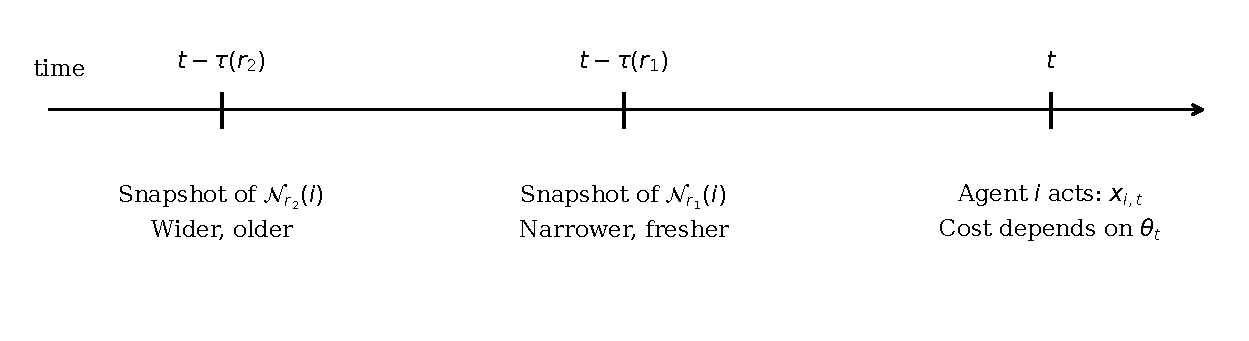
\includegraphics[width=\linewidth]{figures/snapshot_timing.pdf}
\caption{A radius-$r$ synchronized snapshot is taken at time $t-\tau(r)$ and
used for the decision at time $t$. For $r_2>r_1$ with $\tau(r_2)>\tau(r_1)$,
the wider snapshot is older. Cost is evaluated against the current state $\theta_t$.}
\label{fig:snapshot-timing}
\end{figure}
\begin{table}[htbp]
\centering\small
\setlength{\tabcolsep}{3pt}
\caption{Assumptions used in the derivations. All rows use square-integrable
targets and a deterministic positive-definite quadratic cost; normalized shares
require $R_\infty>0$. Entries describe the sufficient assumptions used by the
proofs, including their stated non-Gaussian extensions. ``Fixed epoch'' means
stationarity is unnecessary for that result.}
\label{tab:result-assumptions}
\begin{tabular}{@{}>{\raggedright\arraybackslash}p{.23\linewidth}>{\raggedright\arraybackslash}p{.12\linewidth}>{\raggedright\arraybackslash}p{.13\linewidth}>{\centering\arraybackslash}p{.095\linewidth}>{\centering\arraybackslash}p{.085\linewidth}>{\raggedright\arraybackslash}p{.275\linewidth}@{}}
\toprule
Result & Stationarity & Common-rate innovation & Affine target & Gaussian & Other \\
\midrule
Lemma~\ref{lem:radner_projection}; observation~\eqref{eq:general_crossover}
 & Fixed epoch & No & No & No & Admissible linear policy space \\
Lemma~\ref{lem:innovation_split}; Theorems~\ref{thm:OU_stale_regret}--\ref{thm:local_global_crossover}
 & Time & Yes & Yes & No & Scalar decay; finite-delay crossover as stated \\
Proposition~\ref{prop:aggregate_local}
 & Fixed epoch & No & Yes & No & Independent, mean-zero, equal-variance states \\
Threshold~\eqref{eq:aggregate_rho_star}
 & Time & Yes & Yes & No & Aggregate model plus temporal law \\
Theorem~\ref{thm:spatiotemporal_composition}
 & Time & Yes & Yes & No & Synchronized snapshots \\
Proposition~\ref{thm:marginal_balance}
 & Time & Yes & Yes & No & Differentiable $\tau,\eta_S$; $\eta_S<1$ \\
Lemma~\ref{prop:canonical_eta_S}
 & Space & No & Yes & Yes & $Q=qI$; exponential spatial covariance and kernel \\
Theorem~\ref{thm:canonical_optimal_radius}
 & Space/time & Yes & Yes & Yes & Canonical model and linear delay \\
\bottomrule
\end{tabular}
\end{table}

\clearpage
\section{Marginal-rate illustration}
Figure~\ref{fig:marginal-balance} illustrates how the marginal rates determine the optimal radius for the
canonical model in the main paper.
\begin{figure}[htbp]
\centering
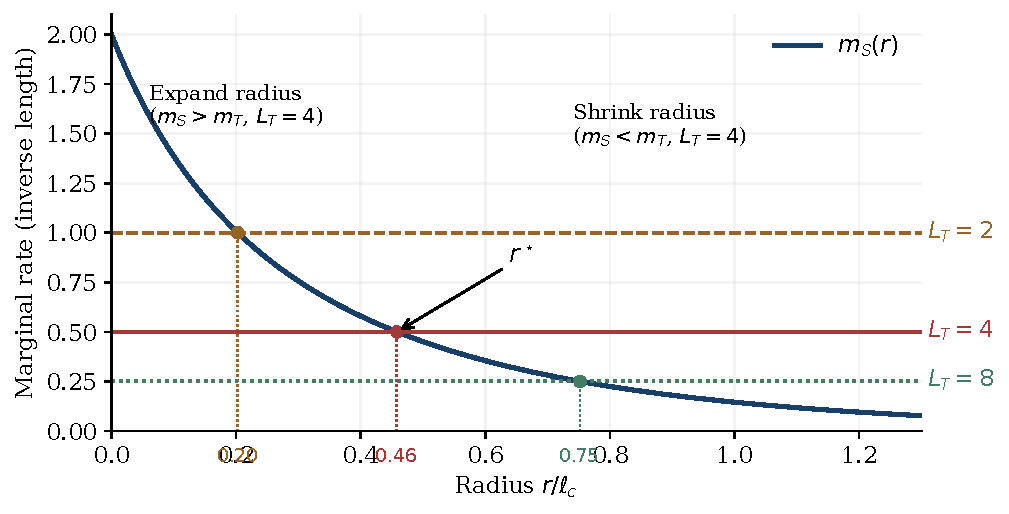
\includegraphics[width=.92\linewidth]{figures/marginal_balance.pdf}
\caption{Marginal balance in the canonical model with $\ell_c=1$ and
$\ell_s=0.5$. Increasing $L_T=vT$ lowers $m_T=2/L_T$ and moves the crossing
with $m_S$ outward. For the middle curve ($L_T=4$), regret falls to the left
of the crossing and rises to its right. This is an illustration of the
analytical rates, not an additional numerical experiment.}
\label{fig:marginal-balance}
\end{figure}


\end{document}
